\documentclass[11pt,a4paper]{article}
%\usepackage{proteins}
%\usepackage{citesupernumber}
%\usepackage{graphics}
\usepackage{overcite}
\usepackage{multirow}
\usepackage{float}
\usepackage{lscape}
%\usepackage{times}
%\usepackage{doublespace}
\usepackage{verbatim}
\usepackage{amsmath}
\usepackage{amstext}
\usepackage{amssymb}
%\usepackage{epsfig}
\usepackage{subfigure}
\usepackage{graphicx}
%\usepackage{epic}
\usepackage{psfrag}
%\usepackage{pstricks}
%\usepackage{eepic}
\usepackage{theorem}
\usepackage{array}
\usepackage{tabularx}
%\usepackage{doublespace}
%\usepackage{calrsfs}
%\usepackage{bibspacing}
%\setlength{\bibspacing}{\baselineskip}
\textwidth 452pt
%\textwidth 26pc
\flushbottom
\textheight 605pt
\topmargin 45pt
\headheight 0pt
\headsep 40pt
\footskip 54pt
\oddsidemargin 0pt
\evensidemargin 0pt
\parindent 0in
\parskip 3ex
\makeatletter
\newcommand\figcaption{\def\@captype{figure}\caption}
    \newcommand\tabcaption{\def\@captype{table}\caption}
\makeatother
   \let\oldthebibliography=\thebibliography
  \let\endoldthebibliography=\endthebibliography
  \renewenvironment{thebibliography}[1]{%
    \begin{oldthebibliography}{#1}%
      \setlength{\parskip}{0ex}%
      \setlength{\itemsep}{0ex}%
  }%
  {%
    \end{oldthebibliography}%
  }
\renewcommand\floatpagefraction{.9}
\renewcommand\topfraction{.9}
\renewcommand\bottomfraction{.9}
\renewcommand\textfraction{.1}
\setcounter{totalnumber}{50}
\setcounter{topnumber}{50}
\setcounter{bottomnumber}{50}
% Math macros
\def\bb{{\mathbf b}}
\def\bx{{\mathbf x}}
\def\bQ{{\mathbf Q}}
\newcommand{\scrB}{\mathcal{B}}
\newcommand{\mbb}{\mathbb}
\newcommand\T{\rule{0pt}{2.6ex}}
\newcommand\B{\rule[-1.2ex]{0pt}{0pt}}


\begin{document}

\section{Introduction}
	Aldolase provides catalysis of the conversion between the hexose 1,6-fructosebisphosphate (1,6FP2) and the two trioses dihydroxy acetone phosphate (DHAP) 
	and glyceraldehyde 3-phosphate (G3P) which is an important reaction within the processes of glycolysis, glucogenesis, and fructose metabolism.  In addition to these
	substrates, aldolase can catalyze the conversion of other phosphorylated sugars including 1-fructose-phosphate (1FP).  Depending on the 
	demands of the tissue that contains the aldolase, aldolase's relative recognition of 1FP and 1,6FP2 must be controlled, which may partially account for
	the fact that humans have three isozymes of aldolase: aldolase A--prominent in muscle tissue, aldolase B--found primarily in the liver, and
        aldolase C--associated with brain tissue.	
	
	The isozymes' Michelis constants ($K_m$) for the cleavage of 1,6FP2 and 1FP have been characterized.  A review of the literature (Kusakabe1994, Motoki1993,
	Kitajima1990, Doyle1995, Berthiaume1993, Malay2002, Pezza(unpublished)) results in 
	the $K_m$'s for 1,6FP2 to be 61 $\pm$ 16 $\mu$\underline{M}, 5 $\pm$ 5 $\mu$\underline{M}, and 11.9 $\pm$ 1.6 $\mu$\underline{M} for human
	aldolase A, B, and C, respectively.  Likewise, the $K_m$'s for 1FP are 42,000 $\pm$ 25,000 $\mu$\underline{M}, 2,500 $\pm$ 1,300 $\mu$\underline{M},
	and 17,000 $\pm$ 1,400 $\mu$\underline{M} for human aldolase A, B, and C, respectively.  Penhoet et al. (Penhoet 1969) also showed that the activity ratio of 
	1,6FP2 to 1FP was approximately 50, 1, and 10 for the orthologous rabbit aldolase A, B, and C.  These results indicate that aldolase overall 
	binds 1,6FP2 stronger than 1FP, that aldolase B has a binding affinity that is approximately a magnitude stronger than aldolase A's, aldolase C binds 
	intermediately between aldolase A and B, and that the preference for 1,6FP2 over 1FP \textit{in vitro} also
	follows this trend with aldolase B showing little or no preference between the two substrates.

	Previous work has noted that the sequences of the three aldolases are all similar having $> 70\%$ pairwise sequence identities.  
	Moreover, aldolase A and C have identical residues within the binding site, and aldolase B has only a single residues, Thr38,
        within the binding site that differs from aldolase A and C, Ser38.  All three isozymes presumably
	have similar catalytic mechanisms, and it is believed that Arg303 in each isozyme, which we investigate wihtin this work, is involved
	in this mechanism (reference?).  This high degree of similarity within these binding sites belies the difference
	in the isozymes' binding profiles, and the biophysical characteristics that result in these profiles still is a question of ongoing interest.

	Our lab has developed a computational tool, FTMap, that can investigate the biophysics of protein interactions (Brenke2009).  Through modeling 
	energetically-favorable positions 
	on the protein for a diverse set of very small molecular probes, regions on the protein surface, termed hot spots, where the protein has a high
	propensity to form
	energetically-favorable interactions with a partner molecule can be identified.  Such hot spots have been experimentally identified using 
	X-ray Crystallography (Allen1996) and Nuclear 
	Magnetic Resonance (Hajduk2005), and such experimental approaches have shown that an effective drug or other strong-binding ligands must form interactions within
	some of the identified hot spots(Mattos1996,Hajduk2005).  While a good theory has not yet been established explaining this correlation, it is reasonable
	to observe that solvated proteins' interactions are dominated by short-range interactions.  Thus pieces of a bound ligand molecule farther from a hot
	spot region than this short-range threshold do not significantly interact with the hot spot suggesting that probes of the size of this 
	threshold should effectively capture the important interactions while reducing the complexity of the overall investigation.  Using such probes,
	FTMap-identified hot spots have been shown to be in good agreement with X-ray crystallography-identified hot spots(Brenke2009)
	as well as known drug molecules (Landon2007,Cheng2009,Hall2012).  In this work, we use FTMap to form a hypothesis concerning the biophysical
	role of the the 45th residue of the three isozymes, and we also use FTMap to investigate the interaction landscape of phosphate containing probes
	to suggest a binding trajectory for the 1,6FP2 within its ring form.

\section{Materials and Methods}

\subsection{Protein structures}
	Protein structures were obtained from the Protein Databank (PDB), www.pdb.org.  All structures analyzed by FTMap were of human aldolase. Mapping was 
	conducted on unbound structures: 2ald for aldolase A, 1qo5 for aldolase B, and 1xfb for aldolase C.  Mapping was also conducted on the K146A mutant
	aldolase A bound to 1,6FP2, 6ald, to investigate the role of this mutation to the binding site mapping results.  Due to the fact that 1xfb is missing
	20 amino acids at its C-terminal region and due to the hypothesis that this region is important in affecting the rate-limiting step of aldolase A, alternative
	forms of 2ald with 20 C-terminal amino acids removed and 1qo5 with 17 C-terminal amino acids removed were mapped.  For the conformational 
	study, 2ald chain A was used for the CTR-bound structure of aldolase A, 1qo5 chain B was used for the CTR-less structure of aldolase B, 1qo5 chain M was
	used for the CTR-bound structure of aldolase B, and 1qo5 chain A was used for the CTR-bound structure of aldolase B that has Phe357 between
	Arg45 and Arg303.
	All structures and FTMap results were visualized using PyMol.

\subsection{Sugar-phosphate structures}
	Sugar-phosphate structure were extracted from bound protein structures obtain from the Protein Databank (PDB), www.pdb.org.  Two structures, 
	from the aldolase A structure 4ald and aldolase B structure 1fdj, of bound 1,6FP2 were taken from the PDB to represent the bound forms of 1,6FP2.  
	As a result of the fact that there does not exist a structure of human aldolase B bound to 1,6FP2, the 1fdj structure of 1,6FP2 bound to rabbit aldolase B, which 
	has a sequence identity of 97\% with human aldolase B, was used to provide an alternative model for the aldolase-bound 1,6FP2.  Due to the fact that
	X-ray results are static while molecules are dynamic \textit{in vivo}, the overlaps of these two bound conformers with the FTMap results using 
	the 16 and 93 probe sets on each of the three aldolases were used to obtain a rough estimate of the occupancy of these two states in each of the 
	three aldolases (see Table 1).  This occupancy was then used in further analysis to obtain an ``averaged " 1,6FP2 structure for each of the aldolases
	including aldolase C which has no bound structure.  The structure for 1,6FP2 from 6ald was also used in our analyses although it was not treated as a biologically 
	relevant binding mode.  The reasoning for this decision is discussed in the ``Results".  Additionally, the two bound conformation of dihydroxy acetone 
	phosphate (DHAP) from 1ado, a structure of rabbit aldolase A  which has 98\% sequence identity with human aldolase A, are 
	treated as biologically relevant binding modes for DHAP in human aldolase A.  

\subsection{Structure alignment}
	All structures were aligned to the unbound, aldolase A structure, 2ald.  Alignment was done on the $\mathrm{C}_\alpha$-carbons of the residues identified
	to be aligned by sequence analysis. 

\subsection{Probe sets}
Two probe sets were used within this investigation (I can provide materials concerning
these probe sets if asked).  The 
first probe set, henceforth the standard set, contains 16 probe molecules that were
initially chosen due to their use in MSCS (Brenke2009).  The seconded probe set,
henceforth the expanded set, contains 93 probe molecules and was developed for the 
purposes of functional-group clustering.  We chose these probes to reflect chemical
moieties commonly found in fragment screening libraries (Hartshorn2005), and
they were chosen by the following two considerations:
\begin{enumerate}
  \item We chose thirteen functional groups: amide, amine, amidine, carboxylic acid, chloride,
    alcohol, fluoride, hydroxamic acid, ether, phenyl, sulfonamide, tetrazole,
    and methyltrifluoride.  From 12 of these compounds we formed 6 probes each by 
    attaching, a methyl, ethyl, isopropyl, isobutyl, furan, or phenyl group.  To the 
    phenyl functional group we only formed 5 probes by attaching a methyl, isopropyl, 
    isobutyl, furan, or phenyl group.  This results in 77 probes with subsets of the probes
    sharing various functional moieties.
  \item We also included additional ring structures since drugs often have ring-like
    moieties.  This included 1-isobutyl
    furan, piperidine, napthalene, 5 nitrogen containing aromatic ring structures, and
    8 nitrogen containing double ring structures.  This results in an additional 16 probes
    that share similar geometry and, in some circumstances, similar chemistry.
\end{enumerate}
The third probe set, known as the phosphate set, follows the construction method of the expanded probe set.
Since aldolase binds molecules with multiple phosphates, the placement of phosphate moieties attached to
various carbon sources is of interest.  Since neither of the other two sets have any phosphate-containing
compounds, a proshphate set of 6 molecules was constructed to model such interaction.

\subsection{Computational solvent sampling}
The premise behind FTMap is that small organic molecules 
of various shapes and polarity consistently interact within
the same vicinities (called hot spots) that contribute large portion
of the binding free energy to a protein-molecule interaction (Hajduk2005,Mattos1996). The solvent 
mapping algorithm in FTMap \cite{Brenke2009} is a direct computational analog of the experimental 
screening technique known as Multiple Solvent Crystal Structures (Allen1996,Mattos1996), and 
FTMap has two sampling stages followed by two stage of cluster 
analysis to model this technique. The individual stages are further detailed in Brenke et al. (2009).
Computational mapping individually places each of the small molecular 
probes on a dense grid around the protein, finds 
favorable positions using empirical free energy functions, and then further minimizes
these positions against the rigid probe for further free energy evaluation. 
For each probe type, the 
individual probes are then clustered and the clusters are ranked on the basis of the 
Boltzmann-averaged 
free energy. Next, consensus clusters are identified as sites in which different probe 
clusters overlap. 

\subsection{Clustering}
	To simulate the favorable location of a single probe, the results for each of the probes from the FTMap results were clustered using the algorithm 
	developed in Brenke et al. (2009).  This algorithm results in a Boltzmann-averaged energy score for each cluster representative, and the representatives 
	with the top six scores are used in further analysis.
	
	To simulate the locations where a diverse set of probes congregate, clustering across probe representatives of all types is done.  The resulting consensus
	sites are ranked by the number of different representatives in the cluster and visualized using PyMol. 

\subsection{Phosphate substructure clustering}
	To obtain an idea where the phosphates tended to migrate in the FTMap results, the representatives obtained after the initial clustering for the 6 probes 
	containing phosphates were further analyzed.  The $CPO_4$ substructure from these
	probes was extracted, and the clustering algorithm was applied to all the $CPO_4$ substructures.  The resulting clusters were ranked by the 
	number of representatives that contributed to the cluster, and the resulting phosphates were visualized with PyMol.

\subsection{Phosphate density visualization} 
The atomic density of the phosphoruses from all probes was placed into a 0.5 \AA\ x 0.5 \AA\ x 0.5 \AA\ grid. All
phosphorus atoms were added to the nearest grid point so that each grid point contained the 
total number of phosphorus atoms within the .125 \AA${}^3$ volume. To account for 
uncertainty in the atomic position as well as to smooth the resulting grid, 
the grid point was convolved 3 times consecutively with a step function that is 
$\frac{1}{27}$ for $i,j,k \in (-1,0,1)$ and 0 everywhere else.
The resulting density was subsequently contoured at the 1 and 3 $\sigma$ levels
using the volume representation within PyMol.

\subsection{Conformation generation}
The steric constraints placed on Arg303 by the different isozymes and Arg45 in aldolase B may be partially responsible for the different
biochemical characteristics of these enzymes.  To investigate the space into which Arg303 may extend within aldolase A
and B and Arg45 in aldolase B, numerous conformations of these arginines were generated (This work was completed by Dmitri Beglov).  Using a
library of arginine coformations taken from the PDB as a starting point, clusters of conformations of arginine were generated.  These
conformations were transposed onto aldolase, and each conformation was minimized in the presence of the static enzyme structure.  
These minimized conformations were then clustered and ranked by energy.  This
minimization process resulted in the resolution of clashes between the arginine and surrounding residues, and the resulting minimized
conformation clusters may be interpretted to represent the region within the protein that Arg303/Arg45 sample while in solution.    

\section{Results}

\subsection{General results}
	Unbound structures of aldolase A, B, and C excluding the C-terminal region (CTR) were mapped for the sake of binding site comparison.  For all maps, the top ranked 
	and most of the highest ranked consensus clusters were found to reside in the active site where 1,6FP2 and 1FP are known to bind in aldolase A and B (see 
	Figure \ref{CTRless}).
	While the results were similar, one observations is worth pointing out.  
	The top ranked consensus clusters migrated to relatively the same position in all three aldolases.  This consensus cluster primarily overlaps the 1- and 2- 
	carbons of the 1,6FP2 models.  In aldolase A and C, this hot spot also extended in a direction essentially perpendicular to these carbons, and additional
	consensus clusters (A's $3^\mathrm{rd}$ ranked consensus cluster and C's $4^\mathrm{th}$ and $6^\mathrm{th}$ ranked consensus clusters) were also found in this vicinity.
	This is in stark contrast with the results for aldolase B which has a conspicuous lack of probes in this perpendicular region possibly due 
	to conformational difference of Arg303 among the isozymes.

\begin{figure}
	\begin{center}
		\mbox
		{
			\subfigure[]{{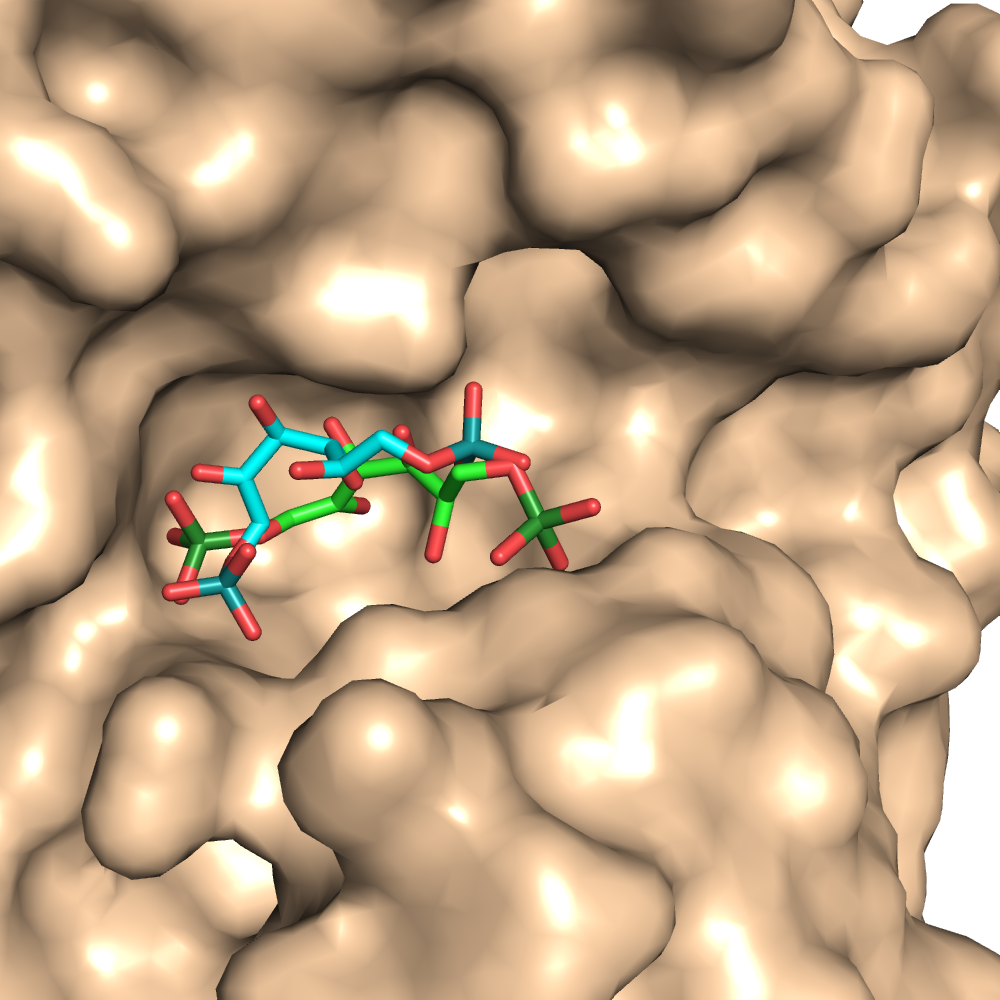
\includegraphics[width=0.5\textwidth]{fig/2ald_m20_and_active_site.png}}\label{active_site}}
			\quad
			\subfigure[]{{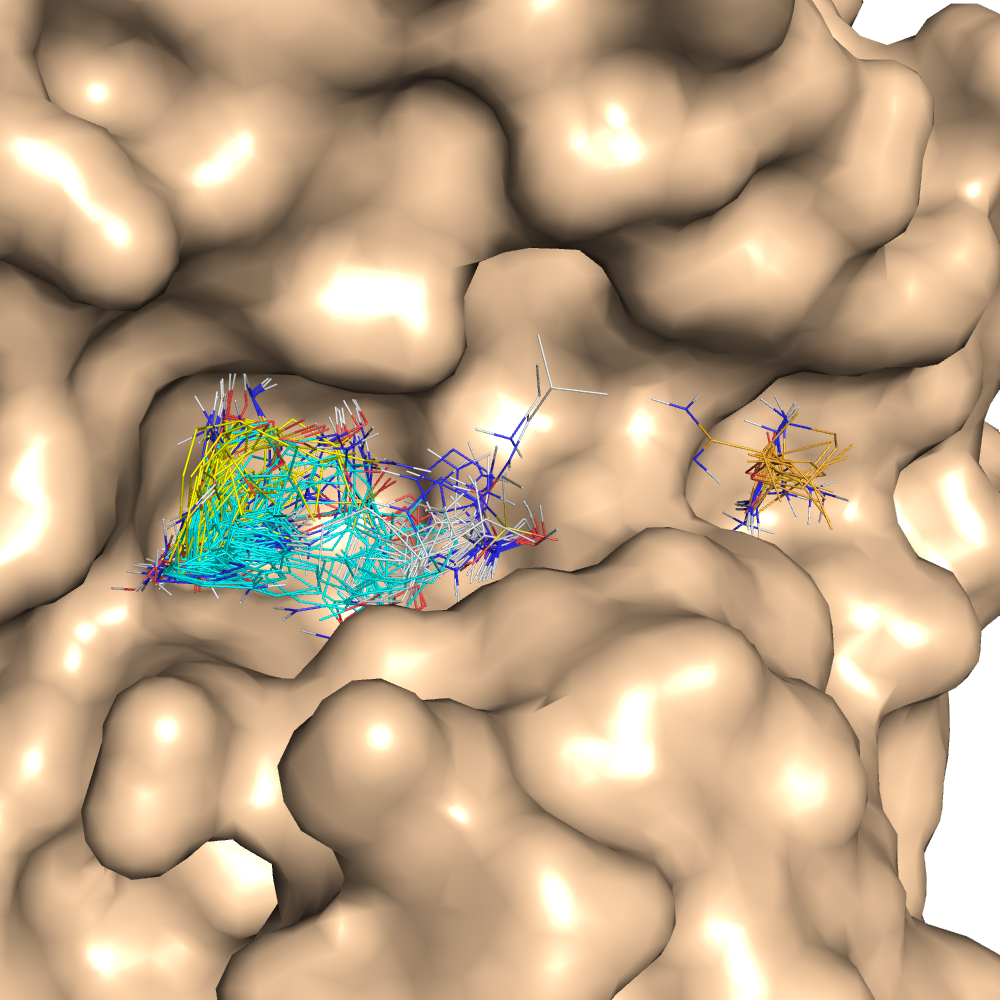
\includegraphics[width=0.5\textwidth]{fig/2ald_m20_and_2ald_m20_clusters.png}}\label{2ald_m20_cc}}
		}
		\mbox
		{
			\subfigure[]{{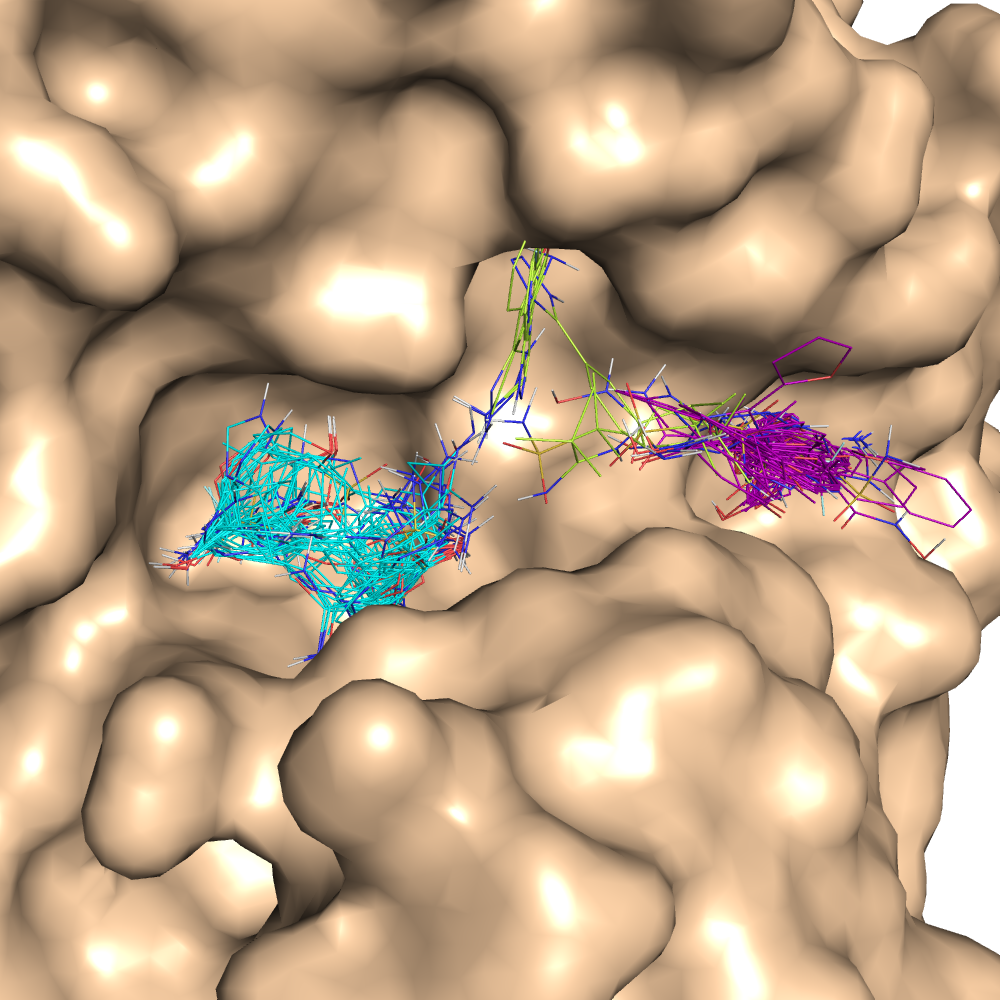
\includegraphics[width=0.5\textwidth]{fig/2ald_m20_and_1qo5_m20_clusters.png}}\label{1qo5_m20_cc}}
			\quad % gives more horizontal spacing
			\subfigure[]{{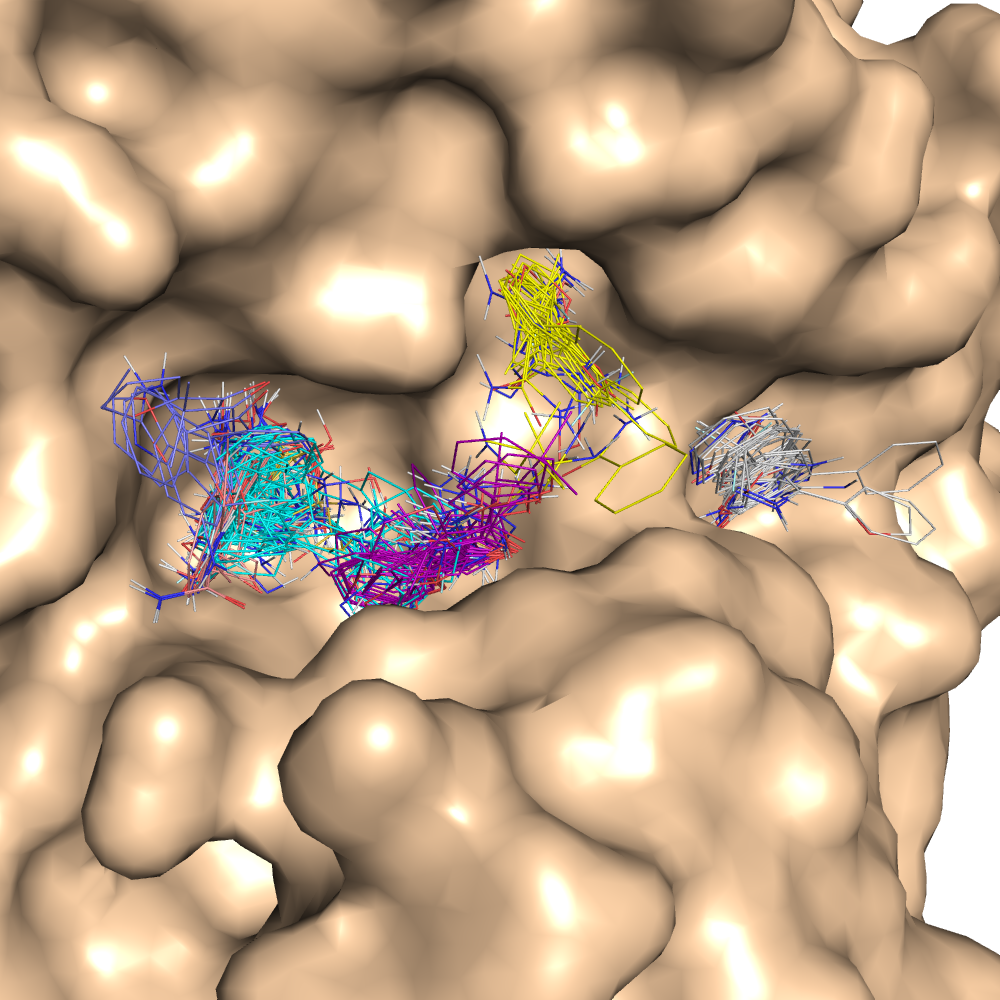
\includegraphics[width=0.5\textwidth]{fig/2ald_m20_and_1xfb_clusters.png}}\label{1xfb_cc}}
		}
		\caption{For all parts, the unbound, aldolase A structure without its CTR (cartoon representation colored wheat)
			was present for the purposes of comparison.  (a.) The bound forms of 1,6FP2 from aldolase A (PDB: 4ald) and rabbit aldolase B (PDB: 1fdj).  
			All oxygens of 1,6FP2 are
			colored red, carbons are colored green and cyan, and phosphates are colored forest green and deep teal for 4ald and 1fdj, respectively.
			(b.-d.)
			Consensus rank corresponds to the following coloring scheme:
			1 cyan, 2 purple, 3 yellow, 4 salmon, 5 white, 6 periwinkle, 7 orange, 8 green, 9 magenta
			(b.)  The results from mapping unbound, aldolase A without its CTR.  (c.)  The results from mapping unbound, aldolase B without its CTR.  
			(d.)  The results from mapping unbound, aldolase C without its CTR. 
		}
		\label{CTRless}
	\end{center}
\end{figure}
	

\subsubsection{The effect of the CTR in aldolase A}
	It has been suggested that the CTR is involved in removing dihydroxy acetone phosphate (DHAP) from the active 
	site in aldolase A (reference); therefore, we mapped and compared
	the results of aldolase A with and without its CTR. Two known conformations of DHAP bound to aldolase A are known from the structure 1ado: one binding in a similar
	position to the known binding of 1,6FP2 from 4ald (green in Figure \ref{CTR}), which we will term the catalytic conformation, and one binding in a similar position to the 
	known binding of 1,6FP2 from the K146A mutant, 6ald (magenta in Figure \ref{CTR}), which we will term the perpendicular conformation.  
	These two conformations of DHAP were then used for orientation and comparison of the results.

\begin{figure}
        \begin{center}
                \mbox
                {
                        \subfigure[]{{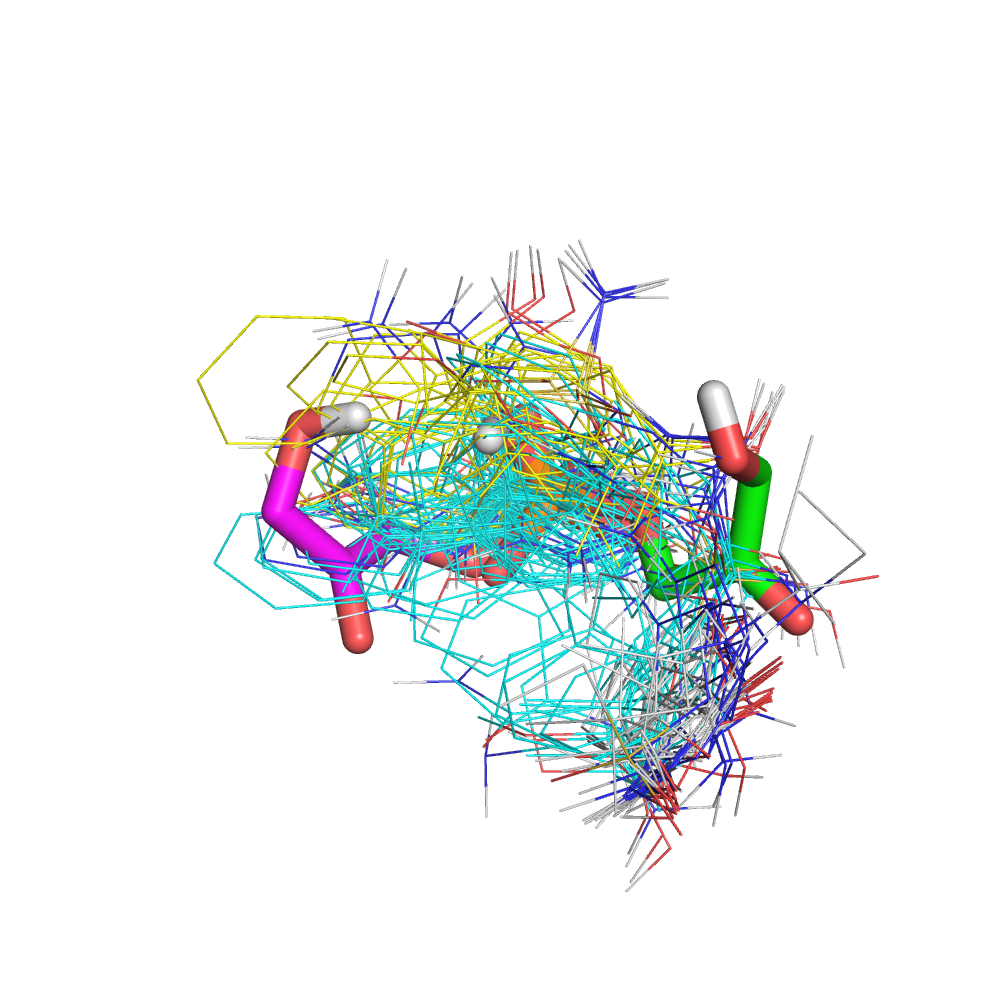
\includegraphics[width=0.5\textwidth]{fig/dhap_and_2ald_m20_clusters.png}}\label{dhap_A_no_CTR}}
                        \quad
                        \subfigure[]{{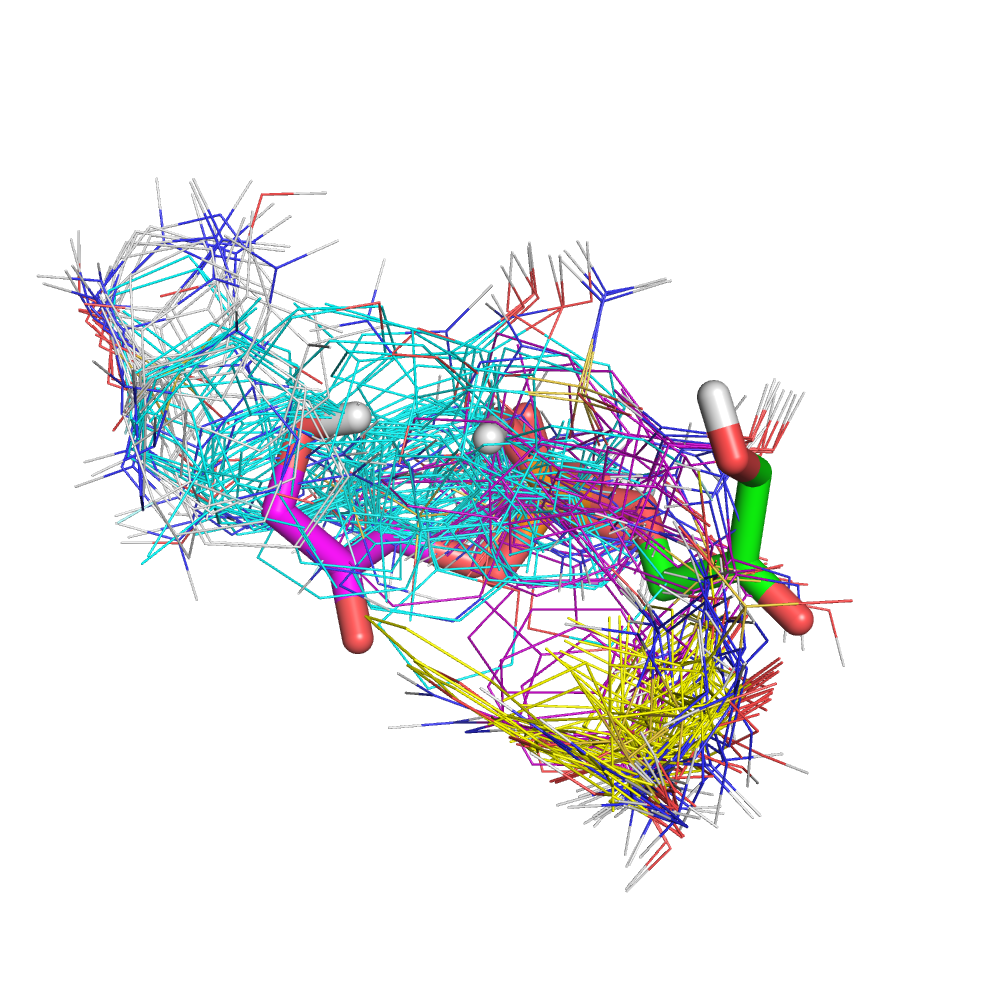
\includegraphics[width=0.5\textwidth]{fig/dhap_and_2ald_clusters.png}}\label{dhap_A_CTR}}
                }
		\mbox
                {
                        \subfigure[]{{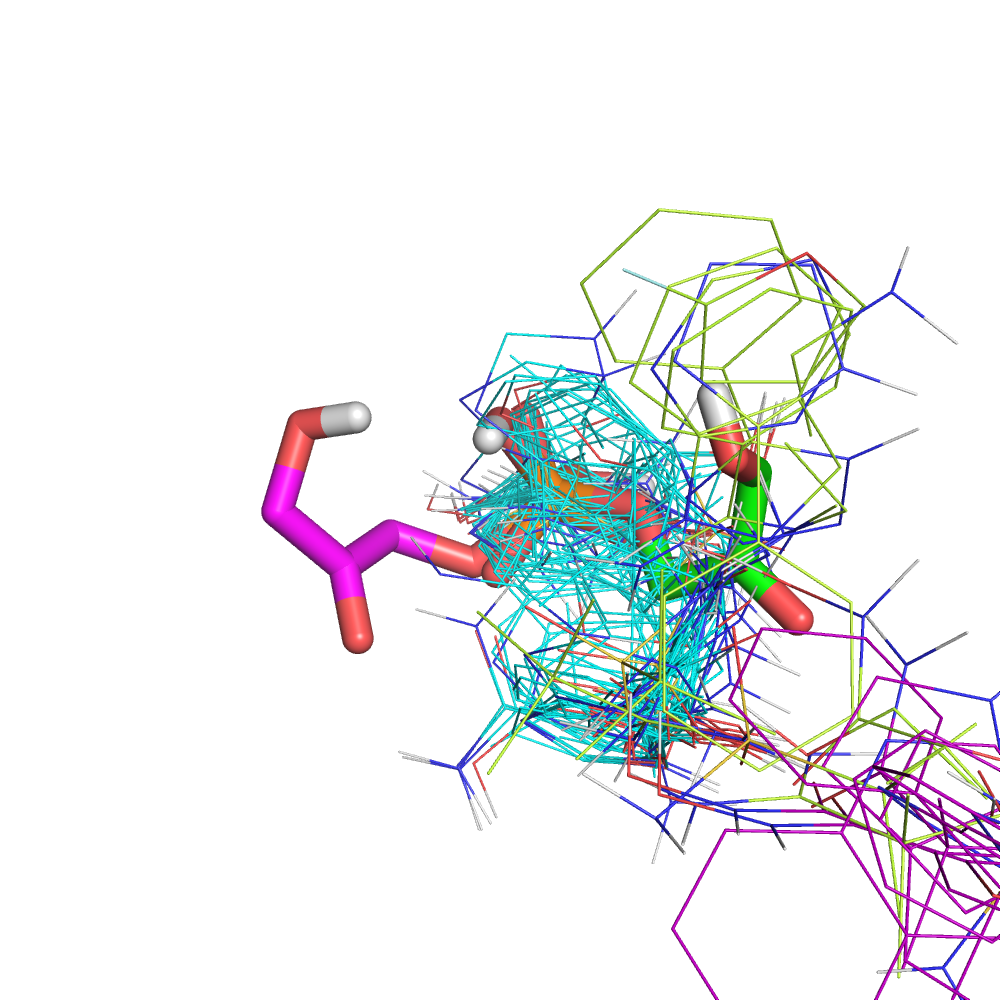
\includegraphics[width=0.5\textwidth]{fig/dhap_and_1qo5_m20_clusters.png}}\label{dhap_B}}
                        \quad
                        \subfigure[]{{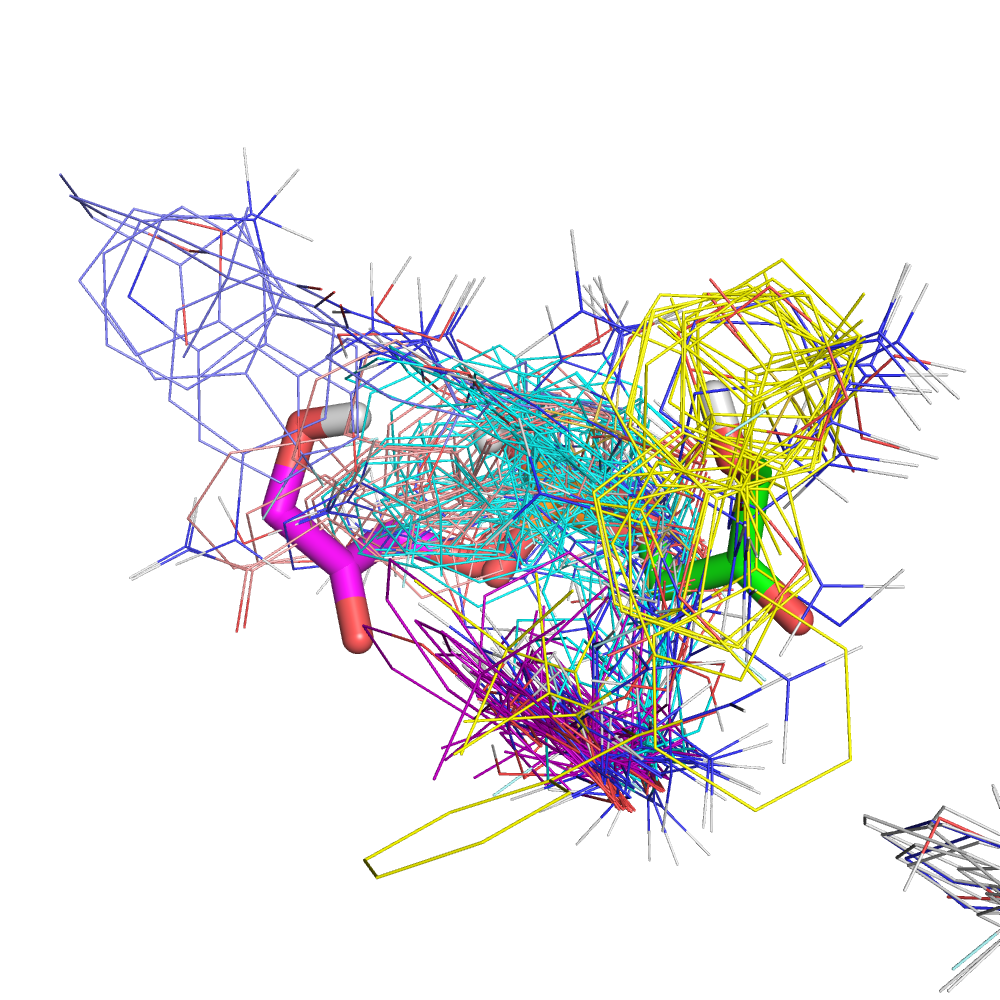
\includegraphics[width=0.5\textwidth]{fig/dhap_and_1xfb_clusters.png}}\label{dhap_C}}
                }
                \caption{
			Dihydroxy acetone (DHAP) from the crystal structure of rabbit aldolase A (1ado) in two conformations (green and magenta).
			Consensus rank corresponds to the following coloring scheme:  1 cyan, 2 purple, 3 yellow,
			4 salmon, 5 white, 6 periwinkle, 7 orange, 8 green
			(a.)  Crossclusters from mapping aldolase A without its CTR superimposed on the DHAP structures.
			(b.)  Crosscluster from mapping aldolase A with its CTR superimposed on the DHAP structures.  Notice that the
			mapping with the CTR has more probes, a different ranking of the crossclusters, and an extension of the top crosscluster
			in the same direction as the magenta DHAP.
			(c.)  Crossclusters from mapping aldolase B without its CTR superimposed on the DHAP structures.  (d.)  Crossclusters from mapping 
			aldolase C without its CTR superimposed on the DHAP structures.
                }
                \label{CTR}
        \end{center}
\end{figure}

	One noticeable difference between the resulting maps from Figure \ref{CTR} is the ranking of the consensus clusters.  
	Specifically, the ranking of the consensus cluster that is primarily in contact with the perpendicular conformation of DHAP is only ranked $3^\mathrm{rd}$ when
	aldolase A does not contain its CTR but is the top ranked cluster when aldolase A does.  
	
	To obtain a quantitative measure of this observation, the number of probe atoms within 2 $\buildrel_{\circ}\over{\mathrm{A}}$
	of the sugar-portion of these conformations was counted, and the ratio of this number from the perpendicular and catalytic conformations was calculated.  
	For the CTR-less form of aldolase A, this ratio is 1.34, and for the aldolase A with its CTR, this ratio was 1.93.  This can be interpreted to mean that 
	the presence of the CTR in aldolase A emphasizes the perpendicular conformation of DHAP thus shifting DHAP away from the catalytic active site.  At this point, 
	it is worth noting that the mapping of aldolase C without its CTR has similar consensus clusters in this region 
	to the mapping of aldolase A without its CTR (compare Figures \ref{dhap_A_no_CTR} and \ref{dhap_C});
	 however, aldolase B has no probes near the perpendicular conformation of DHAP (Figure \ref{dhap_B}) in either of its maps 
	(see Figure \ref{B_comparison}).

\begin{figure}
        \begin{center}
                \mbox
                {
                        \subfigure[]{{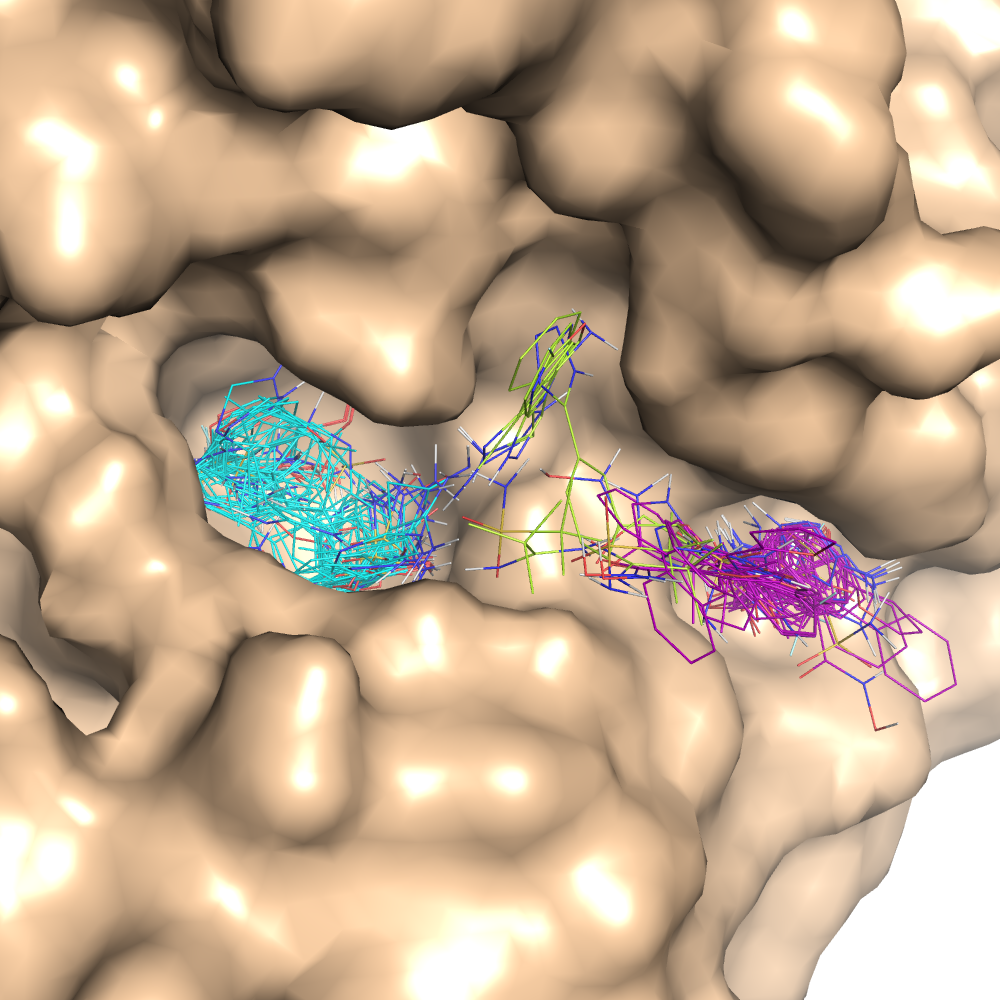
\includegraphics[width=0.5\textwidth]{fig/1qo5_m20_active_site_clusters.png}}\label{B_no_CTR}}
                        \quad
                        \subfigure[]{{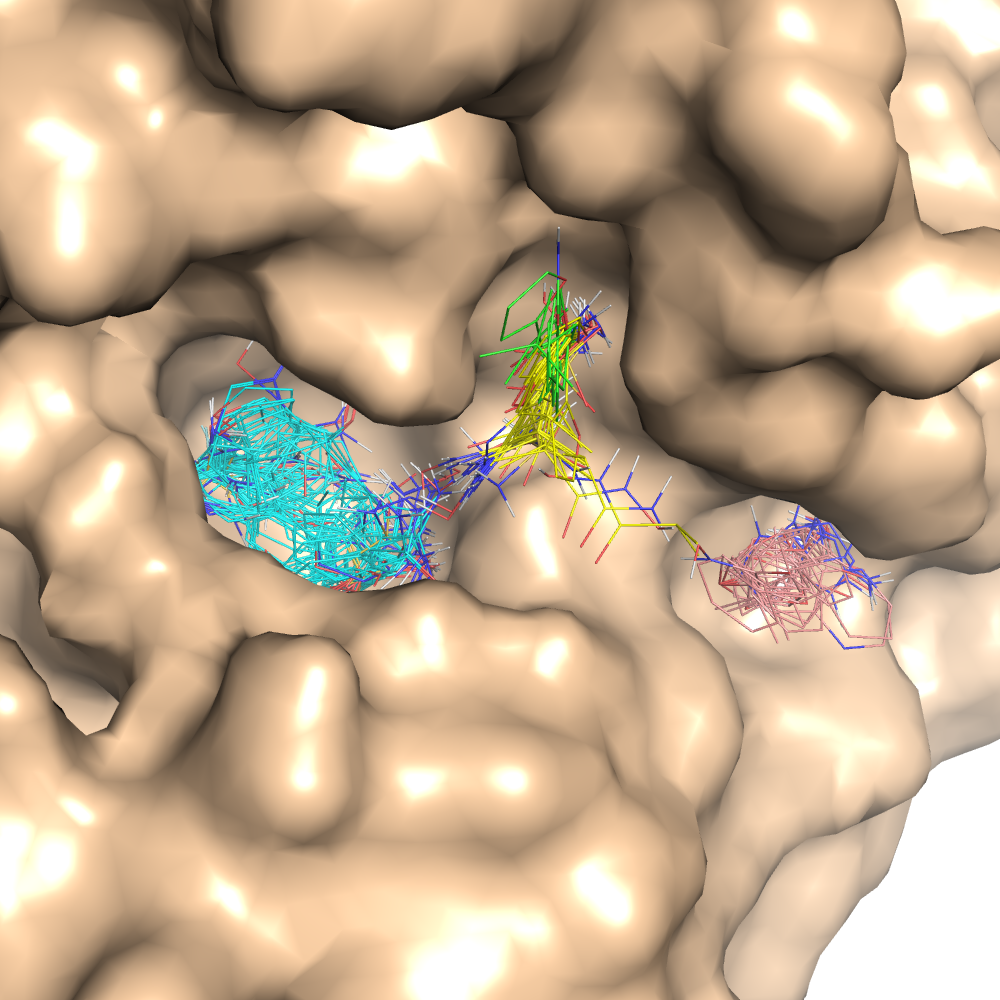
\includegraphics[width=0.5\textwidth]{fig/1qo5_active_site_clusters.png}}\label{B_with_CTR}}
                }
                \caption{Comparison of mapping results between aldolase B with and without its CTR.
                        Consensus rank corresponds to the following coloring scheme:  1 cyan, 2 purple, 3 yellow,
                        4 salmon, 5 white, 6 periwinkle, 7 orange, 8 green.  The protein structure presented as
			a wheat surface is that of 1qo5 missing its terminal 17 amino acids (a.k.a. aldolase B without its CTR).
                        (a.)  The crossclusters within the active site from the mapping of aldolase B without its CTR.
                        (b.)  The crossclusters within the active site from the mapping of aldolase B with its CTR.
                }
                \label{B_comparison}
        \end{center}
\end{figure}


\subsubsection{The effect of the CTR in aldolase B} 
	The role of the CTR in aldolase B was also investigated.  As can be seen in Figure \ref{B_comparison}, the presence of aldolase B's CTR brings more 
	probes and consolidates existing
	probes in the region of the 6-phosphate of 1,6FP2.  Supporting the importance of this region, the phosphate from the bound form of rabbit aldolase B with its CTR is 
	found between the top and $3^\mathrm{rd}$ ranked consensus cluster of human aldolase B with its CTR.  

\subsubsection{Additional consensus regions}
	In addition to the active site, consistent, significant consensus clusters were found in two other locations.  The first additional site is directly next 
	to the active site
	separated by the loop region consisting of residues 270-276.  A consensus cluster was identified in this region in all maps although aldolase B had the largest 
	and highest ranking consensus clusters in this region (ranked $2^\mathrm{nd}$ for aldolase B with the CTR).  
	While most residues were conserved across the three isozymes in this region, a number of positions
	varied (see Table \ref{tab:neighbor}).  Some differences that may be noteworthy include 235, 245, 248, 274, and 278.  These residues
	point into the cavity towards the consensus clusters, and among the three isozymes, aldolase B always has the smallest of the residues at each position.  
	Another difference that may be noteworthy is the Met274 which is unique to aldolase B.  Not only is this residue on the loop that separates the active site from this 
	secondary location, but it is in proximity with Met232 and may be making different interactions with this residue than the glutamines of aldolase A and C.

\begin{table}

\begin{center}
\begin{tabular}{l|c|c|c|}
 & \multicolumn{3}{c}{Amino acid}\\
Position & A & B & C \\
\hline
191 & LEU & LEU & ILE\\
235 & PRO & ALA & PRO\\
240 & THR & THR & PRO\\
241 & GLN & LYS & ILE\\
243 & PHE & TYR & TYR\\ 
244 & SER & THR & THR\\
245 & HIS & PRO & PRO\\
274 & GLN & MET & GLN\\
278 & GLU & ASP & GLU\\
281 & ILE & LEU & PHE 
\end{tabular}
\caption{  Differences in the neighboring site identified by FTMap.  Only residues conserved in all 10 sequences obtained from
	Uniprot for aldolase B are presented.
}\label{tab:neighbor}
\end{center}
\end{table}

	The second consensus region outside the active site was identified on the opposite end of 2 of the beta strands which form the beta barrel and which contribute many
	of the residues which interact with the substrates.  As with the other additional site, all
	maps had a consensus cluster within this region, but aldolase A had multiple and high ranking consensus clusters here (ranked $2^\mathrm{nd}$ and $6^\mathrm{th}$ 
	for aldolase A without the CTR).  Again, most
	residues are the same among the three isozymes, but there are a number of residues that do vary (see Table \ref{tab:back}) which may account for the FTMap result differences.
	Of specific note is position 296 which is alanine in aldolase A and C but lysine in aldolase B.  This residue sits between the two consensus clusters identified in
	aldolase A without the CTR and therefore significantly occludes this cavity in aldolase B. 

\begin{table}

\begin{center}
\begin{tabular}{l|c|c|c|}
 & \multicolumn{3}{c}{Amino acid}\\
Position & A & B & C \\
\hline
20  & HIS & GLN & LEU\\
262 & PRO & ALA & PRO\\
265 & THR & PRO & PRO\\
293 & LYS & LYS & ARG\\
296 & ALA & LYS & ALA\\
338 & CYS & ALA & ALA
\end{tabular}
\caption{  Differences in the back site identified by FTMap.  Only residues conserved in all 10 sequences obtained from
        Uniprot for aldolase A are presented.  Of special interest is residue 296.
}\label{tab:back}
\end{center}
\end{table}

\subsection{Phosphate mapping}
	To further investigate the role of the phosphates within the binding of 
	the 1FP and 1,6FP2 by the different isozymes, phosphate probes were used to map the three isozymes.
	To localize the predicted positions of the phosphates, functional-group clustering was conducted on the six probes containing $CPO_4$ therefore
	isolating this chemical moiety.  The top
	2 phosphate clusters for each isozyme are shown in Figure \ref{phosphate clusters}.  As can be seen in Figures \ref{P A CTR} and 
	\ref{P A no CTR}, the phosphates are best 
	localized near the 1P and 6P phosphates of wild-type 1,6FP2 for aldolase A when the CTR is present and are more diffuse when the CTR is removed.  For aldolase B 
	(Figure \ref{P B no CTR} and \ref{P B CTR}), the 1P site is not present in either map, and the top two sites for the open structure extend towards both
	wild-type and mutant 6P positions while only the wild-type 6P is identified when the CTR is present in aldolase B.  A similar result for 
	the clusters generated by mapping the open aldolase C structure to that of the open aldolase B structure can also be seen in  
	Figure \ref{P C noCTR}.   

\begin{figure}
        \begin{center}
                \mbox
                {
                        \subfigure[]{{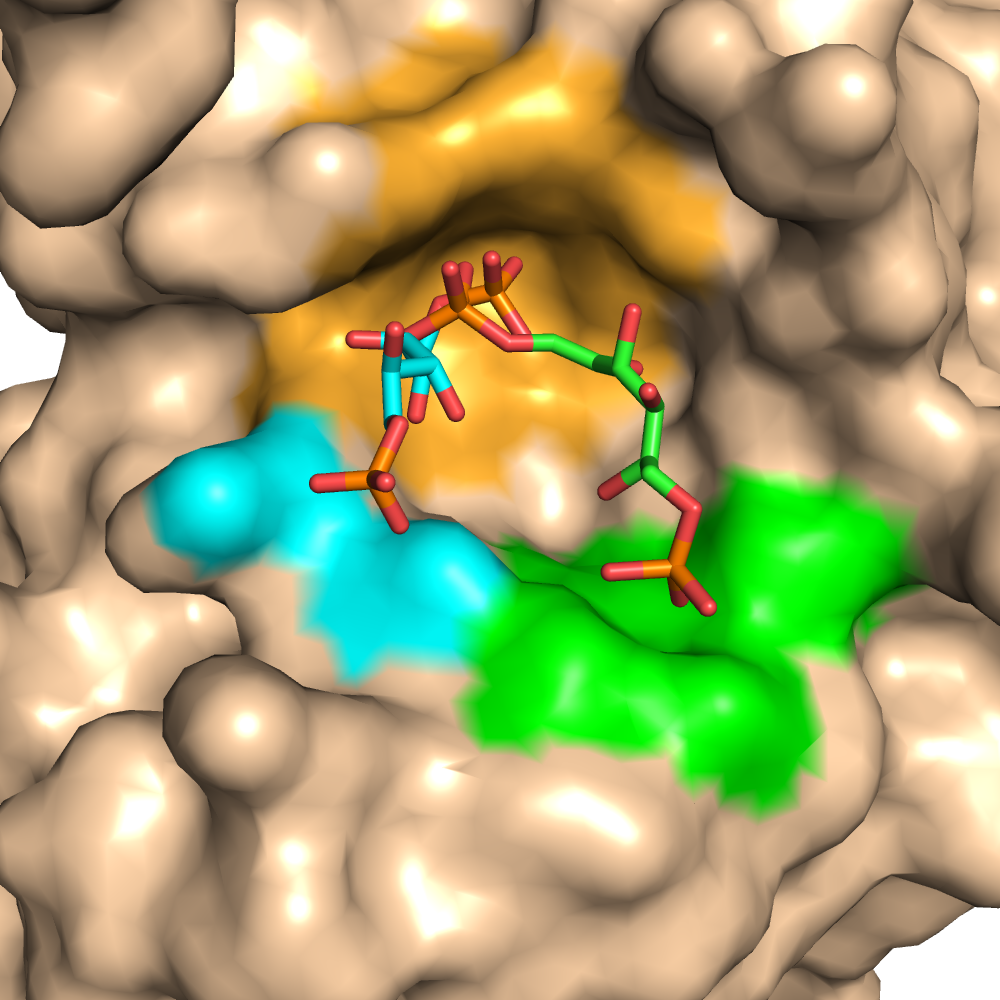
\includegraphics[width=0.3\textwidth]{fig/fbps_and_half_aldolase.png}}\label{P ref}}
                        \quad
                        \subfigure[]{{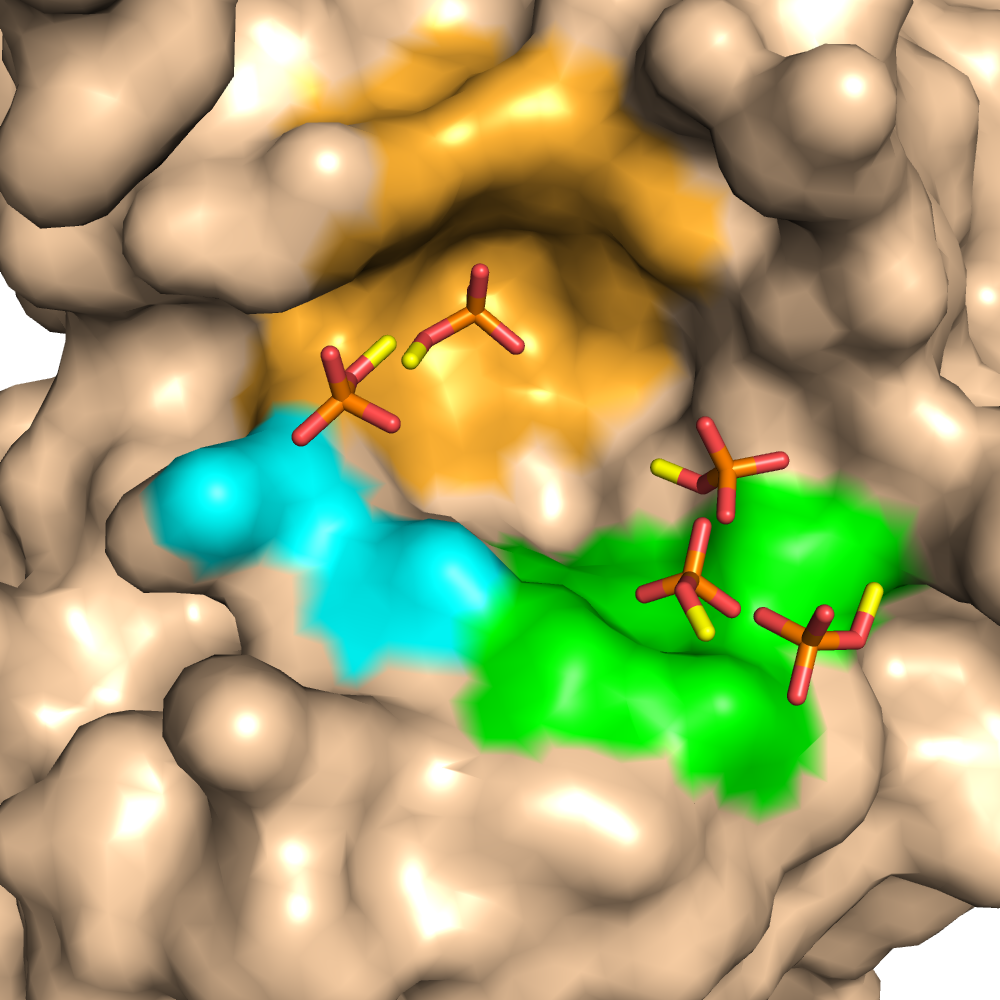
\includegraphics[width=0.3\textwidth]{fig/phosphates_a_open.png}}\label{P A noCTR}}
                        \quad
                        \subfigure[]{{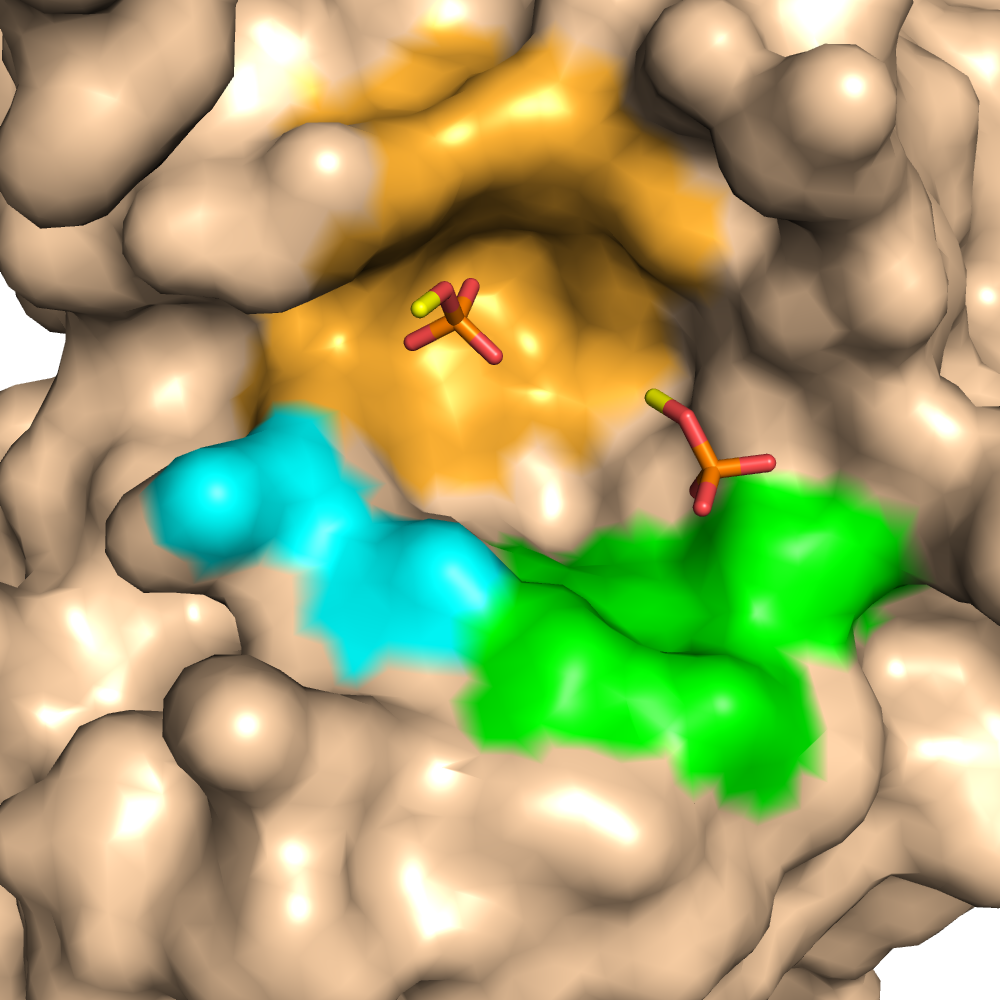
\includegraphics[width=0.3\textwidth]{fig/phosphates_a_closed.png}}\label{P A CTR}}
                }
		\mbox
                {
                        \subfigure[]{{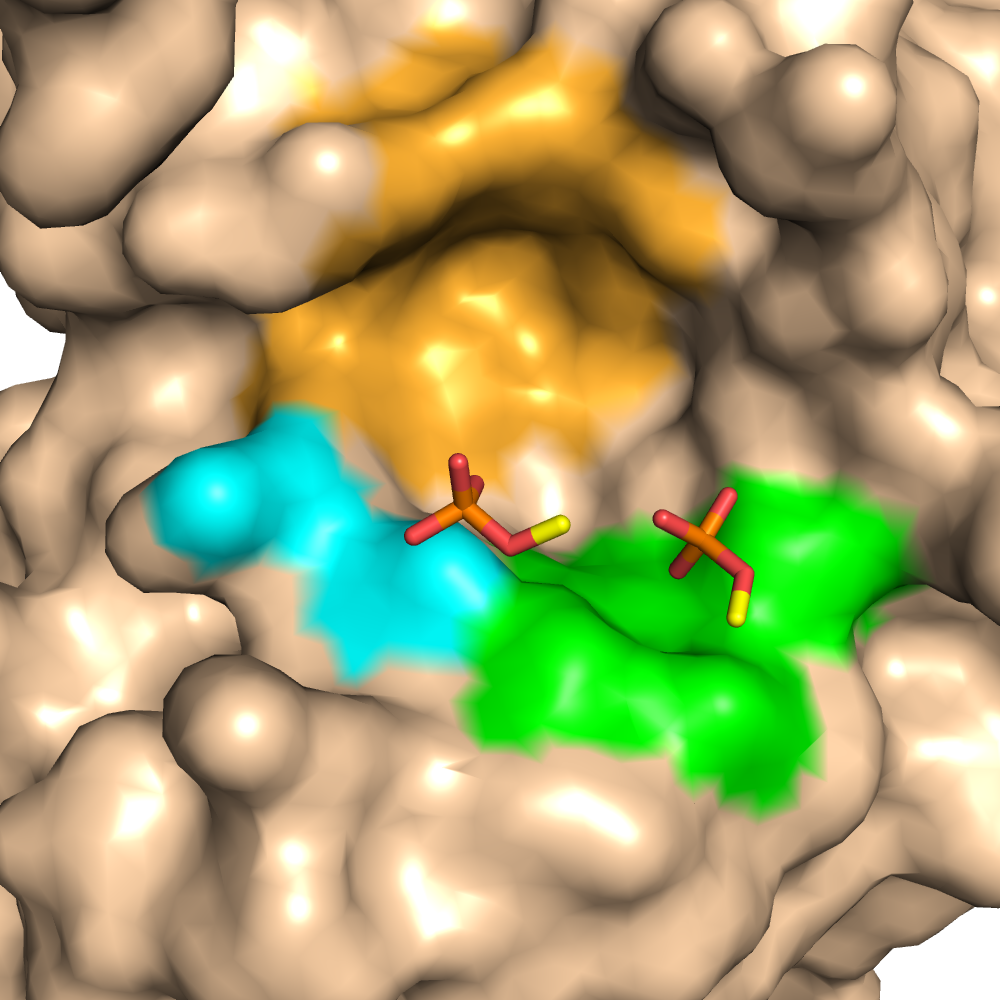
\includegraphics[width=0.3\textwidth]{fig/phosphates_b_open.png}}\label{P B noCTR}}
                        \quad
                        \subfigure[]{{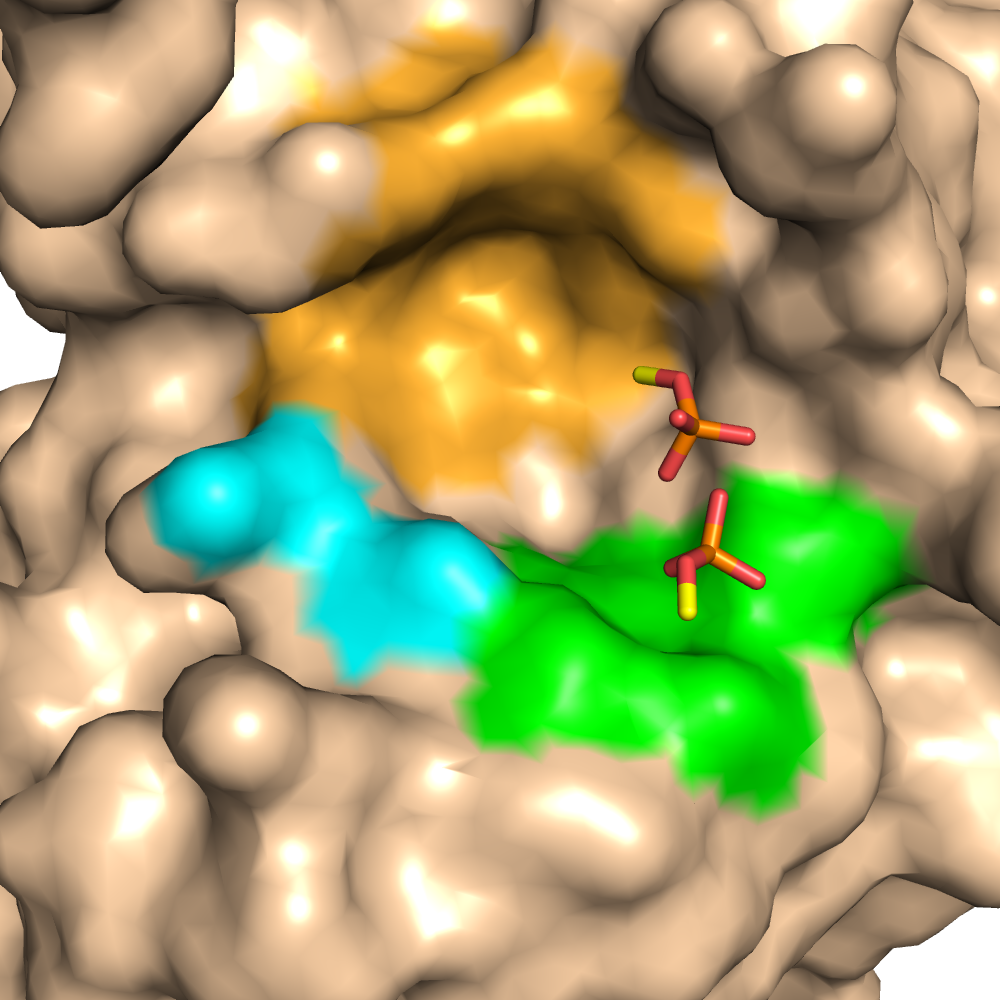
\includegraphics[width=0.3\textwidth]{fig/phosphates_b_closed.png}}\label{P B CTR}}
                        \quad
                        \subfigure[]{{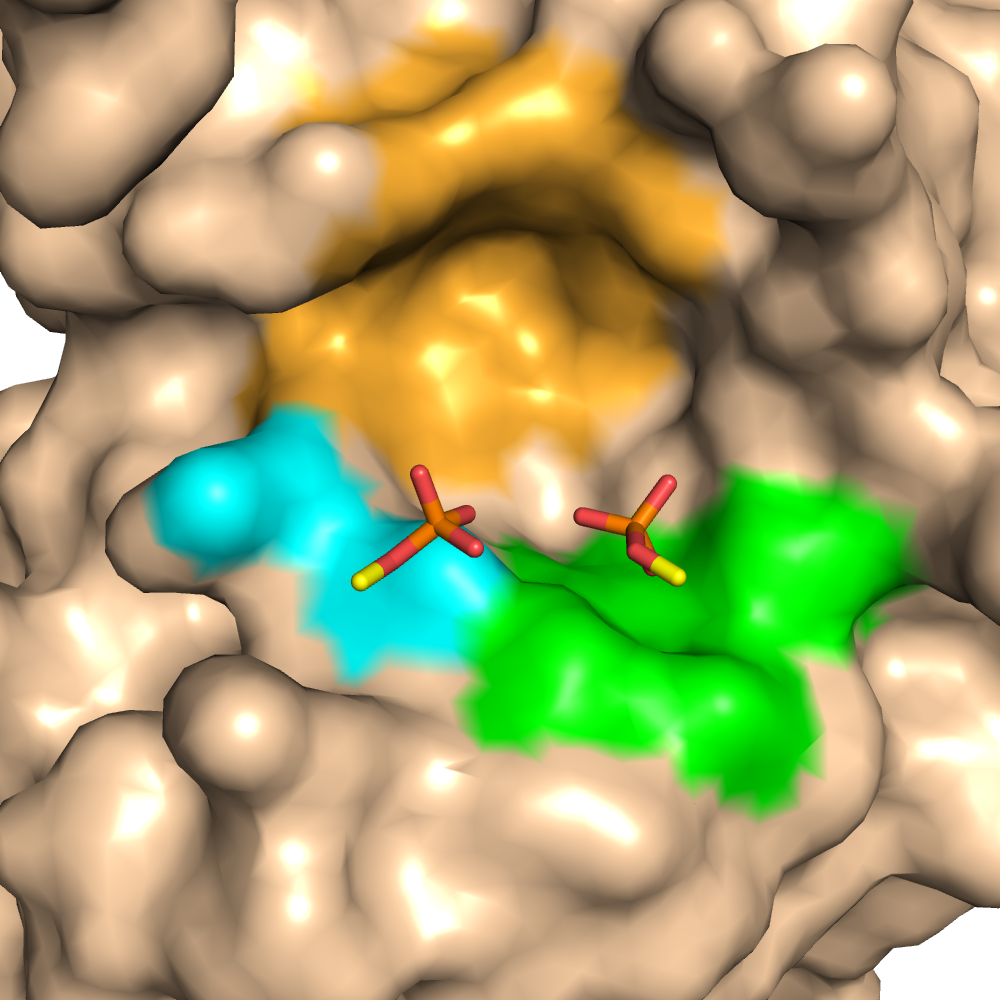
\includegraphics[width=0.3\textwidth]{fig/phosphates_c_open.png}}\label{P C noCTR}}
                }
                \caption{
		Top two phosphate clusters for various mapping results for the three different isozymes.  (a.)
		A portion of the binding pocket of aldolase A (many aldolase residues have been removed to see into the pocket)
		overlayed with bound 1,6FP2 from wild-type structure 4ald (green carbons) and 
		mutant structure 6ald (cyan carbons) for reference.  Aldolase A represented as
		wheat unless it is is within 6 \AA of a phosphate.  If the surface is within 6 \AA of the common phosphate (1P), it is colored orange,
		if it is near the 6P of the wild-type 4ald structure, it is colored green, and if it it near the 6P of the mutant 6ald structure it is colored cyan.
		(b.) The top "two" phosphate clusters for aldolase A without its CTR.  Five clusters are tied for the second-ranked position.
		(c.) The top two phosphate clusters for aldolase A with its CTR. The top two phosphate clusters for aldolase
		B (d.) without and (e.) with its CTR. 	The top two phosphate clusters for aldolase C without its CTR.
                }
                \label{phosphate clusters}
        \end{center}
\end{figure}

	These results suggest that both 6P sites may be present and biologically relevant when the C-terminal region is in its open conformation.
	Since both of these sites are toward the mouth of the binding site versus the fact that the 1P binding site is deep within the pocket and
	since these sites are closer together than either site and the 1P site, it may be the case that the ring structure first binds its two 
	phosphates at both of these sites, and that the 1P site is only used once the ring has been opened.  To further explore the feasibility
	of this hypothesis, a phosphorus density from each of the mapping results of the various forms of the three isozymes was created and
	visualized.  As can be seen in Figure \ref{P den}, the densities of phosphorus atoms seem to trace out two pathways connecting the
	two 6P phosphate sites to the 1P phosphate site.  Consistently, when the structure is open, these pathways extend fully to both 6Ps; however,
	when the CTR closes upon the site, the phosphate site identified by the 6P from the mutant-1,2FP2 bound structure disappears.  This
	observation supports the interpretation both sites are viable when the CTR is open and further suggests that the phosphate bound
	within the mutant 6P binding region moves during the closing of the CTR.   

\begin{figure}
        \begin{center}
                \mbox
                {
                        \subfigure[]{{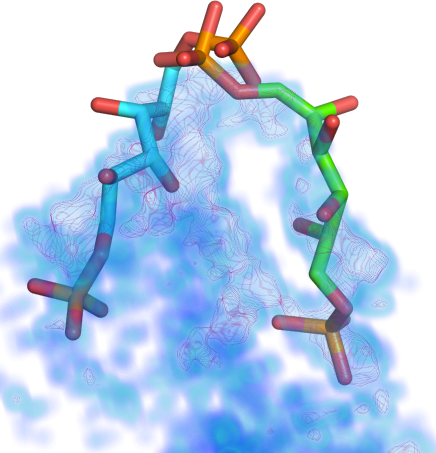
\includegraphics[width=0.3\textwidth]{fig/aldolase_a_open.png}}}
                        \quad
                        \subfigure[]{{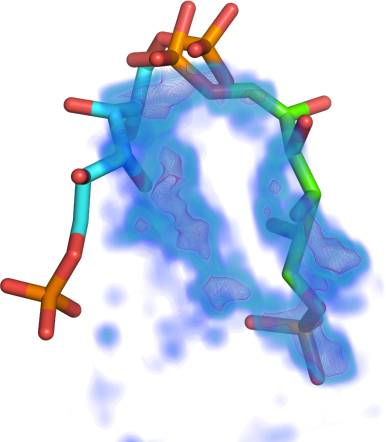
\includegraphics[width=0.3\textwidth]{fig/aldolase_a_closed.png}}}
                }
		\mbox
                {
                        \subfigure[]{{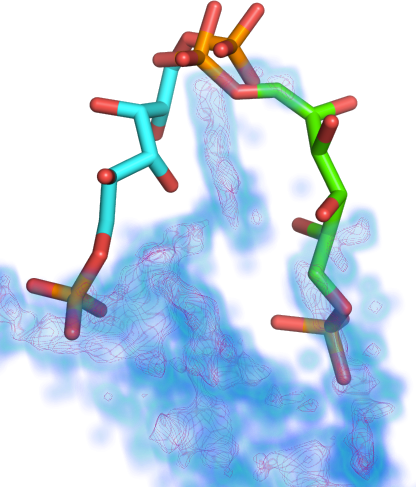
\includegraphics[width=0.3\textwidth]{fig/aldolase_b_open.png}}}
                        \quad
                        \subfigure[]{{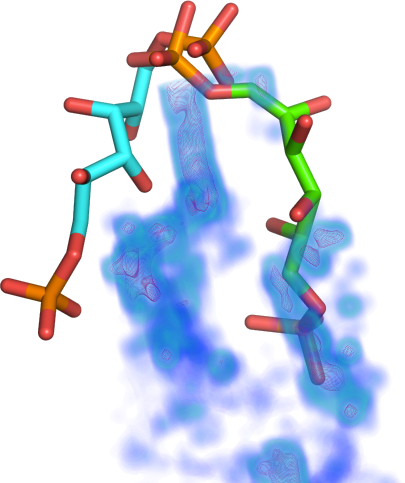
\includegraphics[width=0.3\textwidth]{fig/aldolase_b_closed.png}}}
                        \quad
                        \subfigure[]{{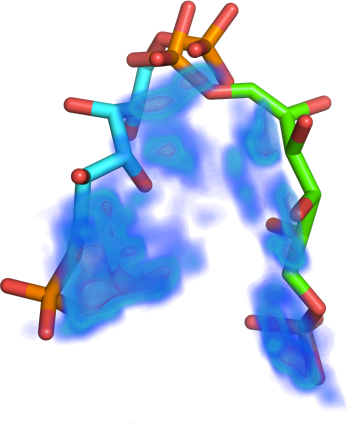
\includegraphics[width=0.3\textwidth]{fig/aldolase_c_open.png}}}
                }
                \caption{
		Densities of phosphorus atoms produced by mapping with phosphate probes.  The densities are contoured at the 
		1 (cyan) and 3 $\sigma$ (red) levels, and colored blue between the 0 and 1 $\sigma$ levels.  1,6FP2 from 
		the wild-type 4ald (green carbons) and mutant 6ald (cyan carbons) structures are shown for comparison (a.)
		A (a.) without and (b.) with its CTR.  
		B (c.) without and (d.) with its CTR. 	(e.) C without its CTR.
                }
                \label{phosphate clusters}
        \end{center}
\end{figure}

\subsection{Conformations of Arg303}
	The differences within the aldolase A, B, and C mapping results near the 1-phosphate binding location suggest different roles
	for Arg303 within these isozymes.  As can be seen by Figure \ref{R303 DHAP}, the alternative form of Arg303 found within aldolase B overlaps with the perpendicular 
	configuration of DHAP observed in DHAP-bound aldolase A.  The aldolase B conformation of Arg303 apparently narrows down this 
	portion of the binding site, and it may largely be responsible for the different behaviors of the two isozymes.  Examination
	of the residues outside of the binding site exposes that
	Arg45 of aldolase B overlaps with the conformation of Arg303
	found within aldolase A and C (see Figure \ref{R45 R303}).  Furthermore, position 45 is differentially conserved among 
	different species as serine in aldolase A and as glutamine 
        in aldolase C suggesting that this residue may be important for differentiating the function of these three isozymes (Tolan's
	previous PhD reference).  In multiple structures of aldolase B, Arg45 adopts the same conformation regardless of the presence or
	absence of a tails, therefore, we hypothesize that Arg45 always restricts the conformational space of Arg303.  

\begin{figure}
        \begin{center}
                \mbox
                {
                        \subfigure[]{{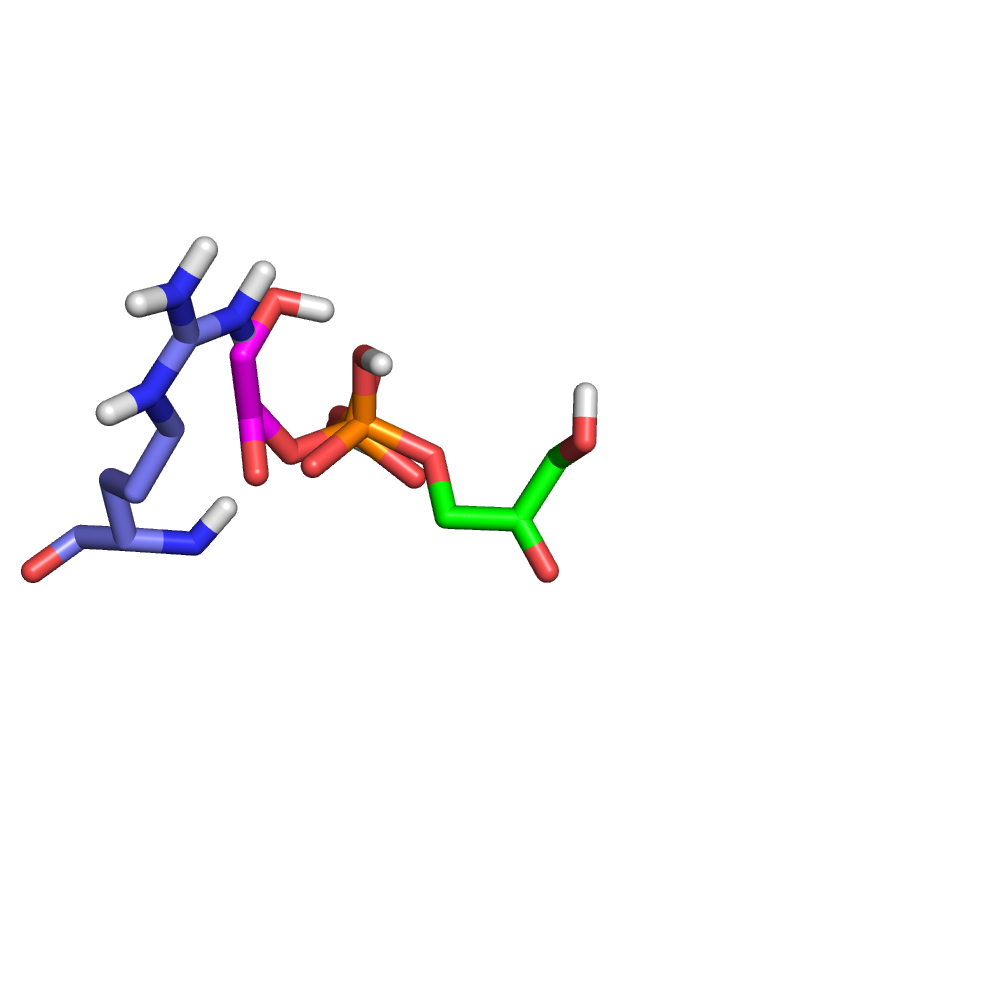
\includegraphics[width=0.5\textwidth]{fig/dhaps_and_arg.png}}\label{R303 DHAP}}
                        \quad
                        \subfigure[]{{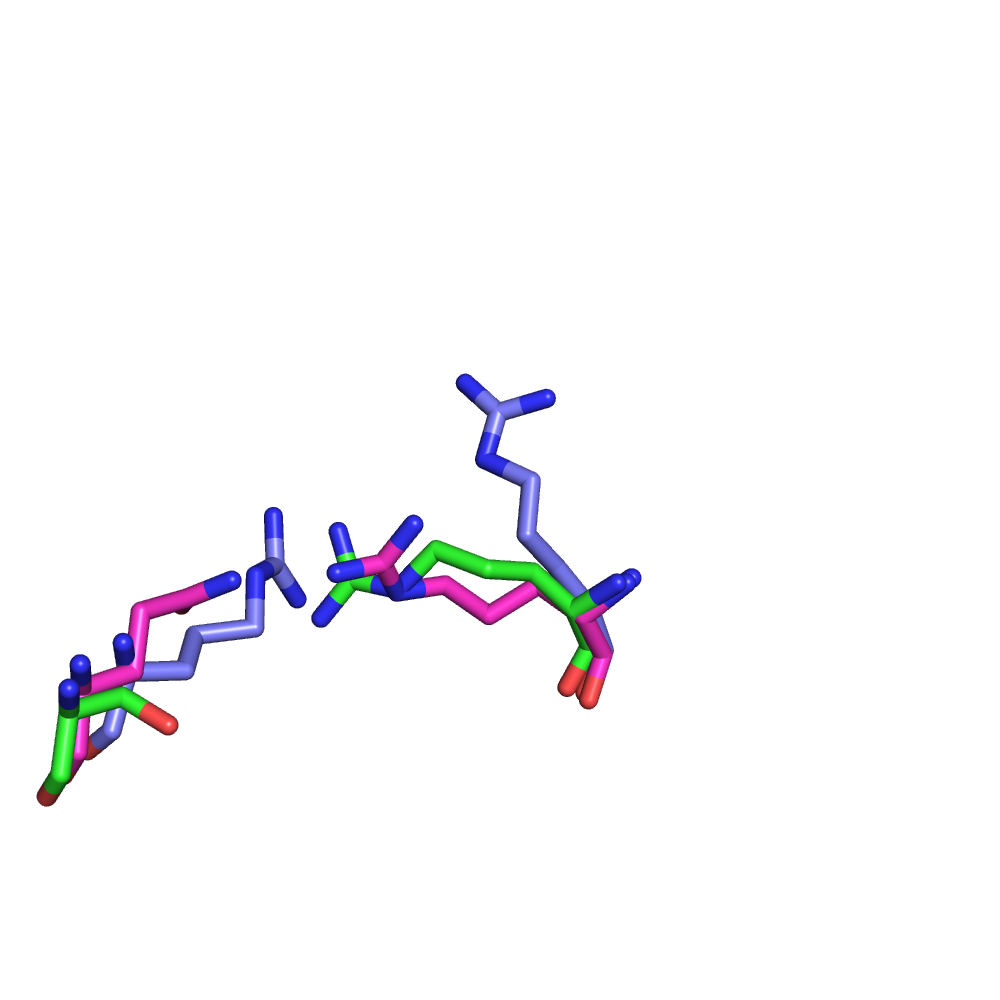
\includegraphics[width=0.5\textwidth]{fig/arg_and_45s.png}}\label{R45 and R303}}
                }
                \caption{(a.) Two conformations of DHAP (green and magenta carbons) bound to aldolase A taken from 1ado superimposed
			upon the conformation of Arg303 (slate carbons) found in adolase B.  (b.)  Position 45 and 303 for aldolase A 
			(green carbons), aldolase B (slate carbons), and aldolase C (magenta carbons).  Position 303 is arginine in all 
			three isozymes, although the conformation of Arg303 is drastically different in B than in A and C.  Position
			45 is serine in aldolase A, arginine in aldolase B, and glutamine in aldolase C.  Notice that Arg45 would clash
			with Arg303 in aldolase B if Arg303 adopted the conformation seen in aldolase A or C.}
                \label{B_comparison}
        \end{center}
\end{figure}

	Furthermore,
	the CTR in both aldolase A and aldolase B has Phe357; however, one structure of aldolase B has Phe357 within a region that is
	between Arg45 and Arg303.  It is not apparent whether Arg45 is necessary to stabilize the restrictive conformation of Phe357 or whether Phe357
	from aldolase A may
	also occupy this conformation but was absent from crystal structures of aldolase A due to crystalization issues, so this difference
	in Phe357 placement may or may not be associated with the differences in biochemical activity between aldolase A and aldolase B.  Regardless,
	Phe357 is part of the CTR and can only be placed next to Arg303 when the tail conformation is closed, thus the placement of this 
	residue within this region may be part of the function of the tail (at least in B), i.e. the placement of Phe357 may be important in regulating
	Arg303 as well.

	To computationally study the roles of Arg45 and Phe357 in restricting the conformational space of Arg303, conformations of Arg303 
	were generated for conformation of aldolase A with its CTR and different conformations of aldolase B (see Figure \ref{conformations}).  
	As can be seen in Figures \ref{conf A} and \ref{conf B noCTR},
	while the top conformation energies of Arg303 from the CTR-bound conformation of Adolase A tend to cluster around the actual bound conformation
	of Arg303, there is also a large confromational region for Arg303 to sample.  The conformation of aldolase B with the CTR has a similar
	region that is slightly restricted by the presence of Arg45 (see Figure \ref{conf B noF}.  This region is further 
	restricted by modeling aldolase B with the CTR that has Phe357 
	in a similar location to that found in the crystal structure of aldolase A.  When the model of aldolase B that has Phe357 placed between 
	Arg45 and Arg303 is used, a highly constricted conformational space
	for Arg303 that corresponds to the bound form of Arg303 in aldolase B is found \ref{conf B F}.
	This suggests that both the presence of Arg45 and Phe357 are important in determining the space within which Arg303 is free to move.
	If this biophysical observation is important for the biochemical functionality of aldolase B, obtaining R45S of aldolase B should result
	in similar catalytic behavior for this mutant as is seen in aldolase A.  Also, it would be interesting to see if F357A may have a somewhat
	milder effect on the catalytic behavior of aldolase B.  Of course, this would need to be compared to a similar mutant in aldolase A.


\begin{figure}
        \begin{center}
                \mbox
                {
                        \subfigure[]{{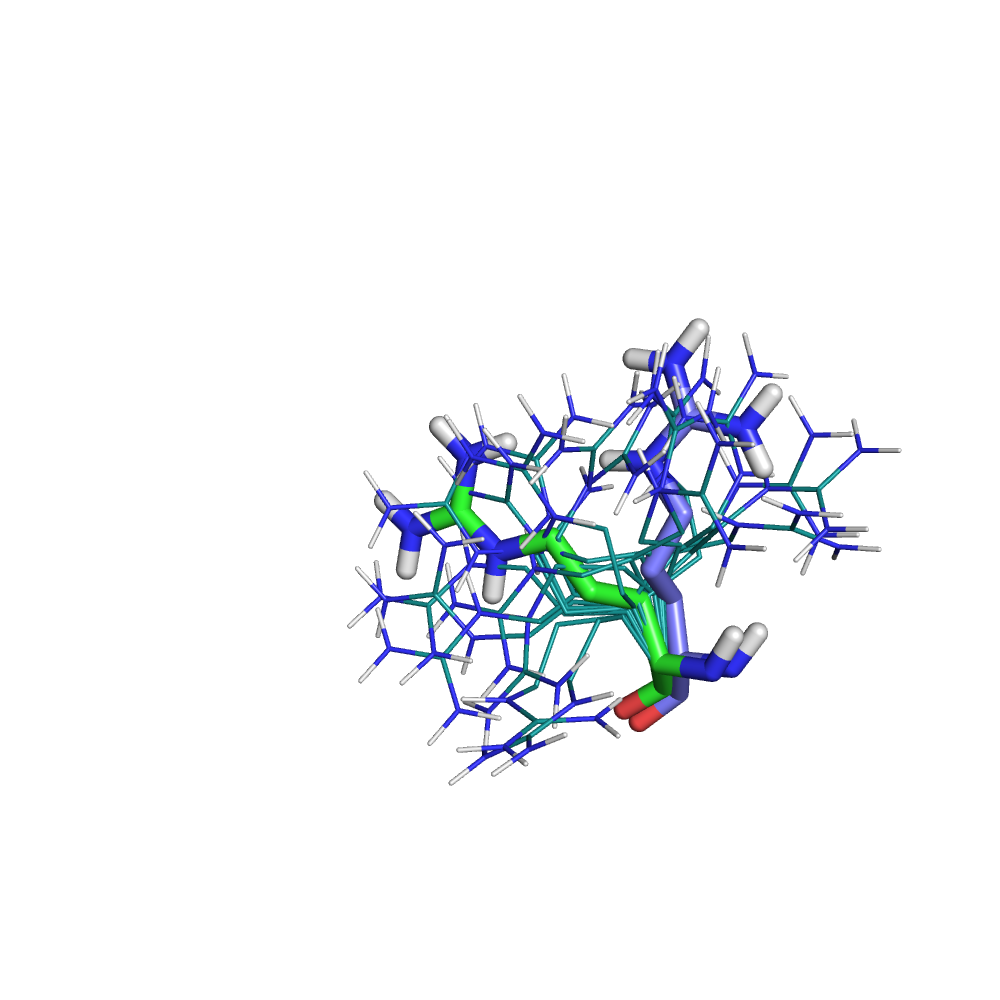
\includegraphics[width=0.5\textwidth]{fig/2ald_303_confs.png}}\label{conf A}}
                        \quad
                        \subfigure[]{{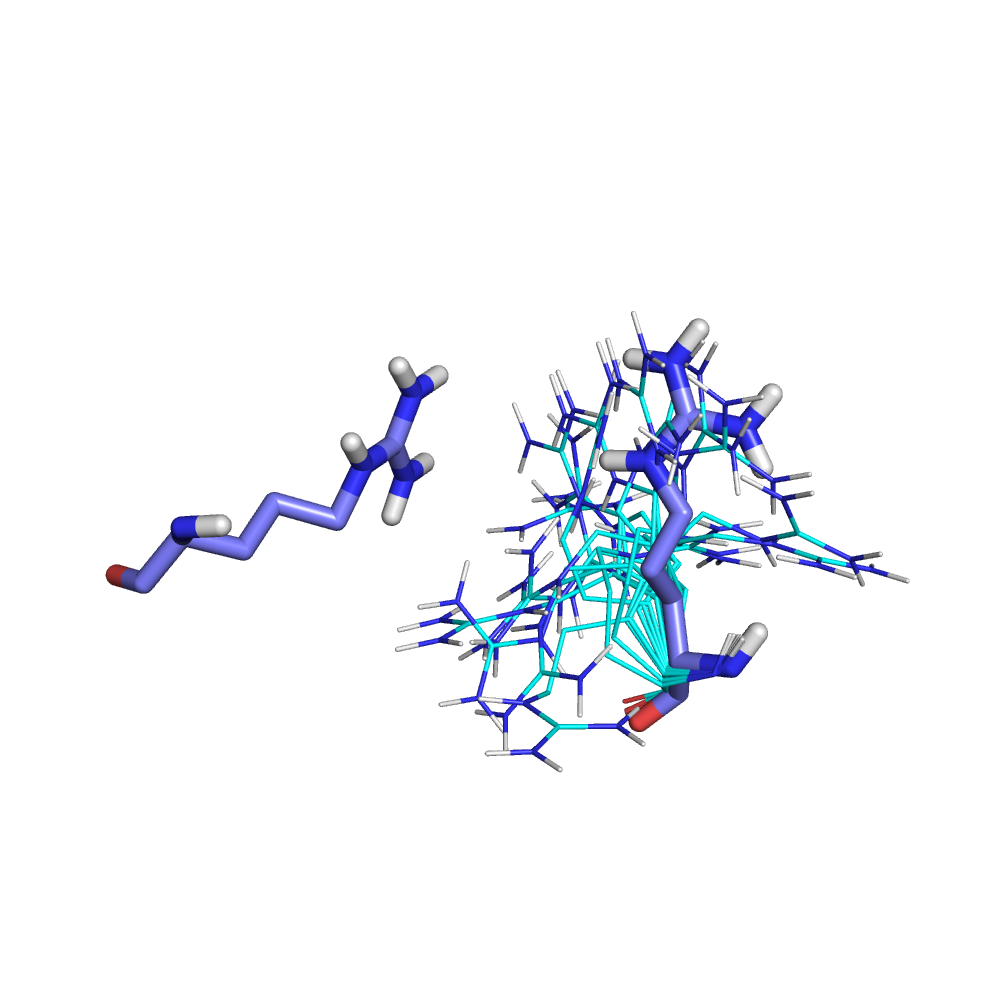
\includegraphics[width=0.5\textwidth]{fig/1qo5_303_confs.png}}\label{conf B noCTR}}
                }
		\mbox
                {
                        \subfigure[]{{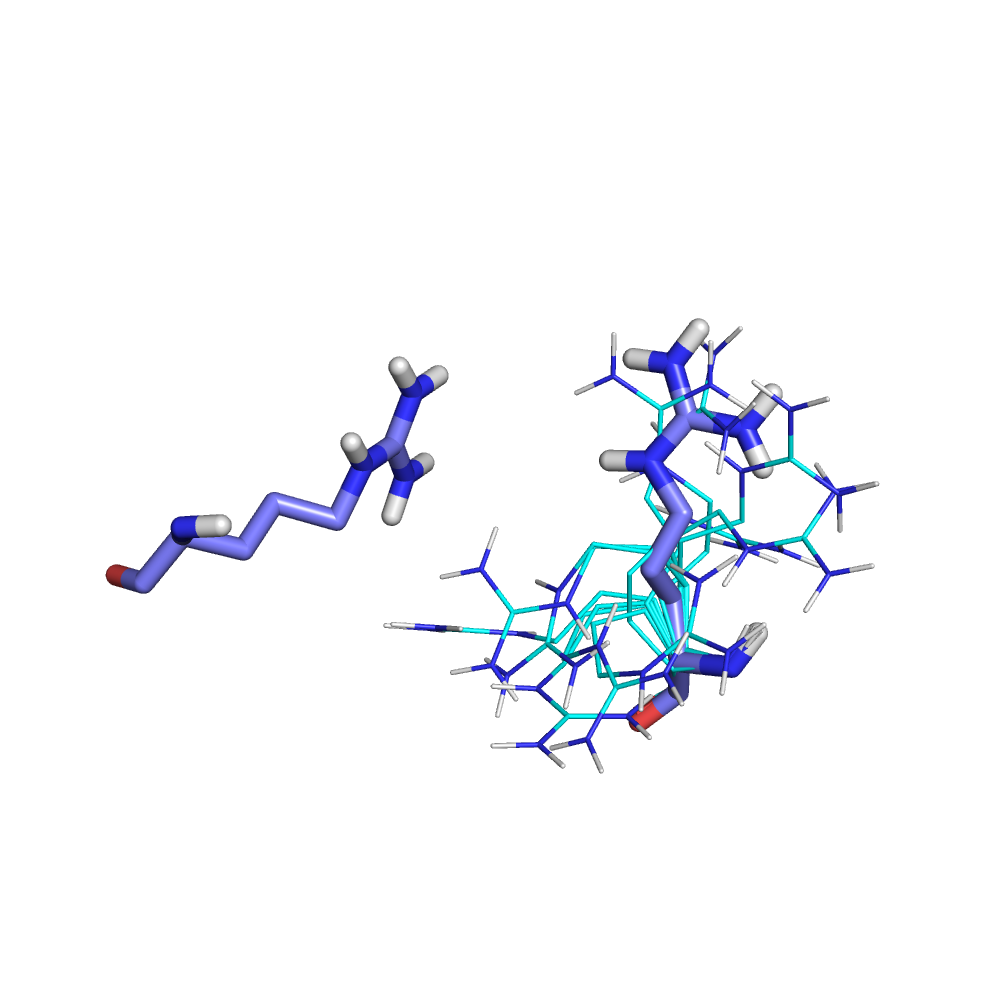
\includegraphics[width=0.5\textwidth]{fig/1qo5_m_confs.png}}\label{conf B noF}}
                        \quad
                        \subfigure[]{{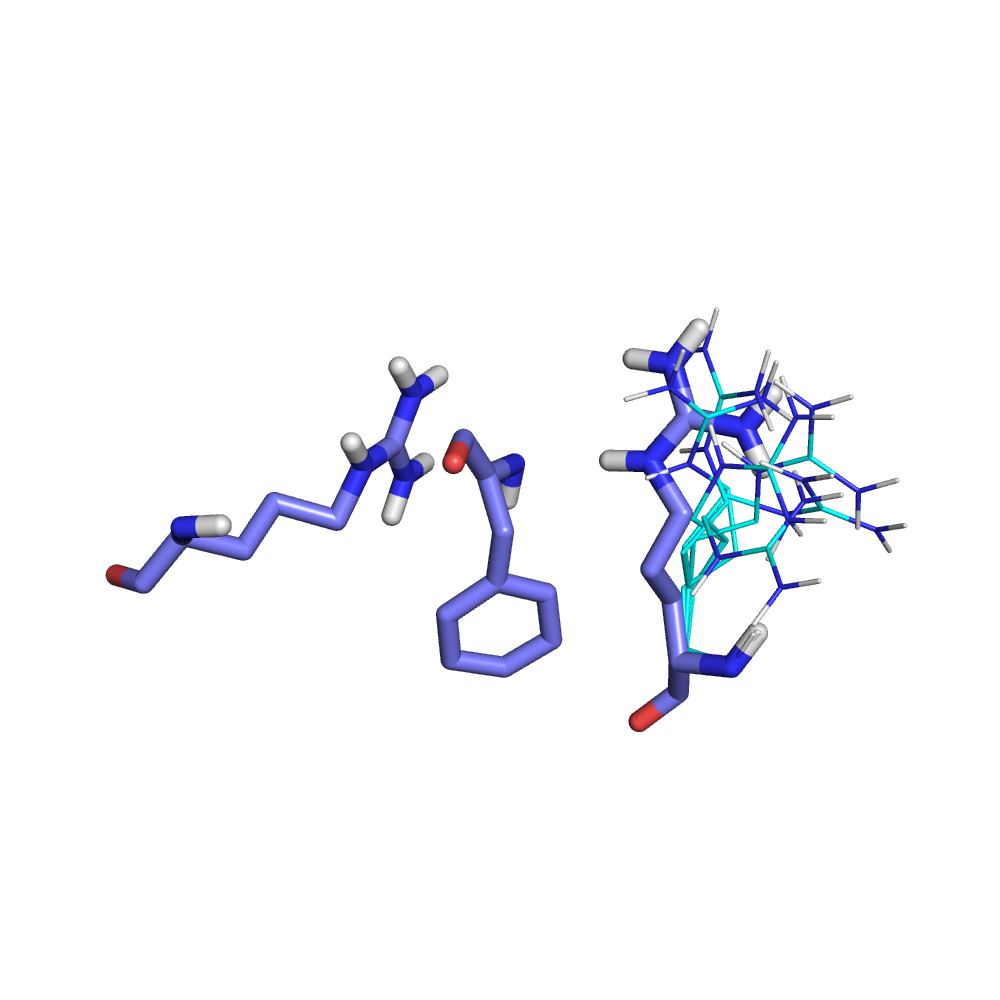
\includegraphics[width=0.5\textwidth]{fig/1qo5_a_confs.png}}\label{conf B F}}
                }
                \caption{
		Modelled conformations of Arg303 in various structures of aldolase. (a.)  Aldolase A with its CTR.  The bound
		conformation of Arg303 from aldolase A is shown as green sticks, the bound conformation of Arg303 from aldolase
		B is shown as slate sticks, and the modeled coformations of Arg303 from Adolase A with its CTR are shown as forest green
		lines. (b.)  Aldolase B with no CTR.  The bound conformation of Arg303 and Arg45 are shown as slate sticks, and the modelled
		conformations of Arg303 are shown as cyan lines.  (c.)  Aldolase B with a conformation of its CTR similar to that of aldolase
		A.  The bound conformation of Arg303 and Arg45 are shown as slate sticks, and the modelled conformations of Arg303 are shown as cyan lines.
		(d.) Aldolase B with a conformation of its CTR that places Phe357 between Arg303 and Arg45.  The bound conformation of Arg303, Arg45, and 
		Phe357 are shown as slate sticks, and the modelled conformations of Arg303 are shown as cyan lines.
                }
                \label{CTR}
        \end{center}
\end{figure}
	

\section{Conclusions}

	
\end{document}
